\documentclass[]{scrartcl}

\usepackage[utf8]{inputenc}
\usepackage[english]{babel}
\usepackage{amsmath}
\usepackage{amsthm}
\usepackage{thmtools}
\usepackage{amssymb}
\usepackage{float}
\usepackage{tikz}
\usepackage{calc}
\usepackage[normalem]{ulem}
\usepackage[framemethod=TikZ]{mdframed}
\usepackage{enumitem}

\usetikzlibrary{arrows}

\newtheorem{theorem}{Theorem}
\newtheorem{lemma}[theorem]{Lemma}
\newtheorem{claim}[theorem]{Claim}
\theoremstyle{definition}
\newtheorem{definition}[theorem]{Definition}

\newcommand{\define}[1]{\uline{#1}}

%System P
\newcommand{\PCons}{\textbf{CONS}}
\newcommand{\Pformulas}{\ensuremath{\mathcal{L}_{(\VarP,\RelP)}}}
\newcommand{\SysP}{\textbf{P}}
\newcommand{\false}{\textbf{false}}
\newcommand{\falses}{\textbf{f}} %false short
\newcommand{\VarP}{\ensuremath{\mathcal{V}_P}}
\newcommand{\RelP}{\ensuremath{\mathcal{P}_P}}
\newcommand{\PModels}{\vdash}
\newcommand{\PModelsf}{\vdash_\text{f}}
%Lambda2
\newcommand{\lambdaTwo}{\ensuremath{\boldsymbol{\lambda2}}}
\newcommand{\lambdaInhab}{\textbf{INHAB}}
\newcommand{\lambdaModels}{\vdash}
\newcommand{\lambdaTypes}{\ensuremath{\text{T}_{\lambda2}}}
\newcommand{\lambdaTerms}{\ensuremath{\Lambda_{\lambdaTypes}}}
\newcommand{\lambdaTypVar}{\ensuremath{\mathcal{V}_T}}
\newcommand{\lambdaValVar}{\ensuremath{\mathcal{V}_V}}
%first-order logic
\newcommand{\rank}{\emph{rk}}
\newcommand{\folmodels}{\ensuremath{\vdash}}
\newcommand{\V}{\text{V}}
\newcommand{\FV}{\text{FV}}
%two-counter automaton
\newcommand{\autHalt}{\textbf{HALT}}
\newcommand{\autStates}{\ensuremath{\mathcal{Q}}}
\newcommand{\autRules}{\ensuremath{R}}
%construction
\newcommand{\conGM}{\ensuremath{\Gamma_{\overline{M}}}}

\makeatletter
\newcommand\getwidthofnode[2]{%
    \pgfextractx{#1}{\pgfpointanchor{#2}{east}}%
    \pgfextractx{\pgf@xa}{\pgfpointanchor{#2}{west}}% \pgf@xa is a length defined by PGF for temporary storage. No need to create a new temporary length.
    \addtolength{#1}{-\pgf@xa}%
}

\long\def\ifnodedefined#1#2#3{%
    \@ifundefined{pgf@sh@ns@#1}{#3}{#2}%
}
\makeatother


%define lengths for tikz
\newlength{\sleft}
\newlength{\sright}

\begin{document}
	\binoppenalty=10000
	\relpenalty=10000
	\tableofcontents
	\begin{sloppypar}
	\newpage
	\section{Introduction}

\subsection{Conventions}
~

$\lambda2$-types: $t, t', t'', t_1, t_2, \dots,s,s_1,s_2,\dots$

$\lambda2$-terms: $M, M', M_1, M_2,\dots, N, N', N_1, N_2, \dots$

first-order terms: 

first-order formulas: $\varphi,\psi,$

type-variables: $\alpha, a, ,\alpha_1, \alpha_2, \dots, \beta, b, \dots$

value-variables: $x, x_1 , x_2 ,\dots$

Predicate-symbols: $P,P^1,P^2,\dots$

\SysP-variables:

\SysP-formulas: $A, B$

two-counter states: $Q,Q',\widehat{Q},Q_f,Q_1,Q_2,\dots$

	\section{Basic Definitions}\label{sec.2}
\subsection{Conventions}
For variable names we will use the following conventions.\\
\lambdaTwo{} types: $t, t', t'', t_1, t_2, \dots,s,s_1,s_2,\dots$\\
\lambdaTwo{} terms: $M, M', M_1, M_2,\dots, N, N', N_1, N_2, \dots$\\
first-order terms: $t,t_1, t_2,\dots$\\
first-order formulas: $\varphi,\varphi_1,\varphi_2,\psi,\psi'$\\
type-variables: $p,p_1,p_2,\alpha, a,\alpha_1, a_1,\alpha_2,a_2, \dots, \beta, b,\beta_1,b_1,\beta_2,b_2, \dots$\\
value-variables: $x,y,z, x_1 , x_2 ,\dots$\\
predicate-symbols: $P,P^1,P^2,\dots$\\
\SysP-variables: $\alpha, a,\alpha_1, a_1,\alpha_2,a_2, \dots, \beta, b,\beta_1,b_1,\beta_2,b_2, \dots$\\
\SysP-formulas: $A,A' ,B,B',A_1,A_2,\dots$\\
states: $Q,Q',\widehat{Q},Q_f,Q_0,Q_1,Q_2,\dots$

If possible we will use Greek letters for bound type-variables and Latin letters for free type-variables.
\subsection{$\boldsymbol{\lambda}$-calculus \lambdaTwo{}}

In the following let $\lambdaTypVar=\{\alpha,a,\beta,b,\dots\}$ be a countably infinite set (of type-variables) and $\lambdaValVar=\{x,x_1,x_2,\dots\}$ be a countably infinite set (of value-variables).
\begin{definition}\label{def.2.1}
	The \define{set of all \lambdaTwo{} types over \lambdaTypVar}, denoted by \lambdaTypes{}, is the smallest set T satisfying the following conditions: %TODO maybe put \lambdaTypVar in \lambdaTypes
	\begin{itemize}
		\item $\lambdaTypVar\subseteq\text{T}$,
		\item if $t_1,t_2\in\text{T}$ then $(t_1\to t_2)\in\text{T}$, and
		\item if $t\in\text{T}$ and $\alpha\in\lambdaTypVar$ then $\forall\alpha.t\in\text{T}$.
	\end{itemize}
	
	The \define{set of all \lambdaTwo{} terms over \lambdaTypVar{} and \lambdaValVar}, denoted by \lambdaTerms{}, is the smallest set $\Lambda_\text{T}$ satisfying the following conditions: %TODO lambda2 explicit
	\begin{itemize}
		\item $\lambdaValVar\subseteq\Lambda_\text{T}$,
		\item if $M_1,M_2\in\Lambda_\text{T}$ then $M_1M_2\in\Lambda_\text{T}$,
		\item if $x\in\lambdaValVar$, $t\in\lambdaTypes$, and $M\in\Lambda_\text{T}$ then $\lambda x:t.M\in\Lambda_\text{T}$,
		\item if $\alpha\in\lambdaTypVar$ and $M\in\Lambda_\text{T}$ then $\Lambda \alpha.M\in\Lambda_\text{T}$, and
		\item if $M\in\Lambda_\text{T}$ and $t\in\lambdaTypes$ then $M\,t\in\Lambda_\text{T}$.
	\end{itemize}
\end{definition}
If we have a type of the form $(t_1\to(t_2\to(\dots \to(t_{n-1}\to t_n)\cdots)))$ we will often omit the brackets and just write $(t_1\to t_2\to\dots\to t_{n-1}\to t_n)$ or $t_1\to t_2\to\dots \to t_{n-1}\to t_n$ instead. %TODO \vec{\alpha}
\begin{definition}\label{def.2.2}
	Let $M,N\in\lambdaTerms$ and $x\in\lambdaValVar$. The \define{substitution of $x$ by $N$ in $M$}, denoted by $M\left[x:=N\right]$ is defined as follows:
	\[M\left[x:=N\right]=
		\begin{cases}
			N                     & \text{if $M=x$}                \\
			y                     & \text{if $M=y$ and $y\neq x$}  \\
			(M_1\left[x:=N\right])(M_2\left[x:=N\right])  & \text{if $M=M_1M_2$}           \\
			\lambda x:t.M'        & \text{if $M=\lambda x:t.M'$}   \\
			\lambda y:t.(M'\left[x:=N\right])             & \text{if $M=\lambda y:t.M'$ and $y\neq x$}   \\
			\Lambda\alpha.(M'\left[x:=N\right])           & \text{if $M=\Lambda\alpha.M'$} \\
			(M'\left[x:=N\right])\,t                      & \text{if $M=M'\,t$}            \\
		\end{cases}\]
	Let $t,t'\in\lambdaTypes$ and $a\in\lambdaTypVar$. The \define{substitution of $a$ by $t$ in $t'$}, denoted by $t\left[a:=t'\right]$ is defined as follows:
	\[t\left[a:=t'\right]=
		\begin{cases}
			t'                    & \text{if $t=a$}                    \\ 
			b                     & \text{if $t=b$ and $b\neq a$}      \\ 
			(t_1\left[a:=t'\right])\to (t_2\left[a:=t'\right])  & \text{if $t=t_1\to t_2$}           \\
			\forall a.t''         & \text{if $t=\forall a.t''$}\\
			\forall\beta.(t''\left[a:=t'\right]) & \text{if $t=\forall\beta.t''$ and $\beta\neq a$}\\
		\end{cases}\]
		
	Let $M\in\lambdaTerms$, $a\in\lambdaTypVar$, and $t\in\lambdaTypes$. The \define{substitution of $a$ by $t$ in $M$}, denoted by $M\left[a:=t\right]$ is defined as follows:
	\[M\left[a:=t\right]=
		\begin{cases}
			x                                             & \text{if $M=x$}  \\
			(M_1\left[a:=t\right])(M_2\left[a:=t\right])  & \text{if $M=M_1M_2$}           \\
			\lambda x:t'\left[a:=t\right].(M'\left[a:=t\right])             & \text{if $M=\lambda x:t'.M'$}   \\
			M                                             & \text{if $M=\Lambda a.M'$} \\
			\Lambda\beta.(M'\left[a:=t\right])           & \text{if $M=\Lambda\beta.M'$ and $\beta\neq a$} \\
			(M'\left[a:=t\right])\,t\left[a:=t\right]     & \text{if $M=M'\,t$}            \\
		\end{cases}\]
\end{definition}

In the following we will often abbreviate $(\dots(M\left[a_n:=b_n\right])\dots)\left[a_1:=b_1\right]$ to $M\left[\vec{a}:=\vec{b}\right]$ where $\vec{a}=a_1\dots a_n$ and $\vec{b}=b_1\dots b_n$.

\begin{definition}\label{def.2.3}
	Let $M\in\lambdaTerms$. The \define{set of free variables of $M$}, denoted by $\FV(M)$, is defined inductively as follows:
	\[\FV(M)=
		\begin{cases}
			\{x\}                 & \text{if $M=x$}                \\
			\FV(M_1)\cup\FV(M_2)  & \text{if $M=M_1M_2$}           \\
			\FV(M')\setminus\{x\} & \text{if $M=\lambda x:t.M'$}   \\
			\FV(M')               & \text{if $M=\Lambda\alpha.M'$} \\
			\FV(M')               & \text{if $M=M'\,t$}            \\
		\end{cases}\]
			
	The \define{set of bound variables of $M$}, denoted by $\GV(M)$, is defined as follows:
	\[\GV(M)=
		\begin{cases}
			\emptyset             & \text{if $M=x$}                \\ 
			\GV(M_1)\cup\GV(M_2)  & \text{if $M=M_1M_2$}           \\
			\GV(M')\cup\{x\}      & \text{if $M=\lambda x:t.M'$}   \\
			\GV(M')               & \text{if $M=\Lambda\alpha.M'$} \\
			\GV(M')               & \text{if $M=M'\,t$}            \\
		\end{cases}\]
\end{definition}

\begin{definition}\label{def.2.4}
	Let $t\in\lambdaTypes$. The \define{set of free type-variables of $t$}, denoted by $\FV(t)$, is defined inductively as follows:
	\[\FV(t)=
		\begin{cases}
			\{a\}                 & \text{if $t=a$}                    \\ 
			\FV(t_1)\cup\FV(t_2)  & \text{if $t=t_1\to t_2$}           \\
			\FV(t')\setminus\{\alpha\} & \text{if $t=\forall\alpha.t'$}\\
		\end{cases}\]
	The \define{set of bound type-variables of $t$}, denoted by $\GV(t)$, is defined inductively as follows:
	\[\GV(t)=
		\begin{cases}
			\emptyset              & \text{if $t=a$}                    \\ 
			\GV(t_1)\cup\GV(t_2)  & \text{if $t=t_1\to t_2$}           \\
			\GV(t')\cup\{\alpha\} & \text{if $t=\forall\alpha.t'$}
		\end{cases}\]	
\end{definition}

Now we can lift this definition to terms.

\begin{definition}\label{def.2.5}
	Let $M\in\lambdaTerms$. The \define{set of free type-variables of $M$}, denoted by $\TFV(M)$, is the union of all sets of free type-variables of types occurring in $M$.
	
	The \define{set of bound type-variables of $M$}, denoted by $\TGV(M)$, is the union of all sets of bound type-variables of types occurring in $M$.
	%defined inductively as follows:
%	\[\TFV(M)=
%		\begin{cases}
%			\emptyset                   & \text{if $M=x$}                \\
%			\TFV(M_1)\cup\TFV(M_2)      & \text{if $M=M_1M_2$}           \\
%			\TFV(M')\cup\FV(t)          & \text{if $M=\lambda x:t.M'$}   \\
%			\TFV(M')                    & \text{if $M=\Lambda\alpha.M'$} \\
%			\TFV(M')\cup\FV(t)          & \text{if $M=M'\,t$}            \\
%		\end{cases}\]
			
%	The \define{set of bound type-variables of $M$}, denoted by $\GV(M)$, is defined as follows:
%	\[\TGV(M)=
%		\begin{cases}
%			\emptyset              & \text{if $M=x$}                \\ 
%			\TGV(M_1)\cup\TGV(M_2) & \text{if $M=M_1M_2$}           \\
%			\TGV(M')\cup\GV(t)     & \text{if $M=\lambda x:t.M'$}   \\
%			\TGV(M')               & \text{if $M=\Lambda\alpha.M'$} \\
%			\TGV(M')\cup\GV(t)     & \text{if $M=M'\,t$}            \\
%		\end{cases}\]
\end{definition}

\begin{definition}\label{def.2.6}
The \define{$\beta$-reduction}, denoted by $\lambdaB$, is a binary relation on $\lambdaTerms$. For all $M,N\in\lambdaTerms$, $x\in\lambdaValVar$, $t\in\lambdaTypes$, and $\alpha\in\lambdaTypVar$ if $\GV(M)\cap\FV(N)=\emptyset$ then $(\lambda x:t.M)N\lambdaB M\left[x:=N\right]$ and from $\TGV(M)\cap\TFV(N)=\emptyset$ it follows that $(\Lambda\alpha.M)t\lambdaB M\left[\alpha:=t\right]$.

The \define{$\alpha_1$-conversion}, denoted by $\lambdaAO$, is a binary relation on $\lambdaTerms$. For all $M\in\lambdaTerms$, $x,x'\in\lambdaValVar$, $t\in\lambdaTypes$, and $\alpha,\beta\in\lambdaTypVar$ if $x'\notin\FV(M)\cup\GV(M)$ then $\lambda x:t.M\lambdaAO\lambda x':t.(M\left[x:=x'\right])$ and from $\beta\notin\TFV(M)\cup\TGV(M)$ it follows that $\Lambda \alpha.M\lambdaAO\Lambda \beta.(M\left[\alpha:=\beta\right])$.

The \define{$\alpha_2$-conversion}, denoted by $\lambdaAT$, is a binary relation on $\lambdaTypes$. For all $t\in\lambdaTypes$, and $\alpha,\beta\in\lambdaTypVar$ if $\beta\notin\FV(t)\cup\GV(t)$ then $\forall\alpha.t\lambdaAT\forall\beta.(t\left[\alpha:=\beta\right])$.
\end{definition}

Note that right now we are not able to reduce terms within a context (e.g there is no $M\in\lambdaTerms$ such that $\lambda x:t.(\lambda y:t.y)x\lambdaB M$).

\begin{definition}\label{def.2.7}
So, for a binary relation $\rightarrow$ on \lambdaTerms{} we define the \define{closure of $\rightarrow$ under term contexts}, denoted by \lambdaTermContext{\rightarrow}, as the smallest binary relation $\Rightarrow$ on \lambdaTerms{} containing $\rightarrow$ such that for all $N,M,M'\in\lambdaTerms$, $x\in\lambdaValVar$, $t\in\lambdaTypes$, and $\alpha\in\lambdaTypVar$. If $M\Rightarrow M'$ then
\begin{align*}
MN&\Rightarrow M'N      & \lambda x:t.M&\Rightarrow\lambda x:t.M' & M\,t&\Rightarrow M'\,t \\
NM&\Rightarrow NM'   & \Lambda\alpha.M&\Rightarrow \Lambda\alpha.M'   
\end{align*}
also hold.

For a binary relation $\rightarrow'$ on \lambdaTypes{} we define the \define{closure of $\rightarrow'$ under type contexts}, denoted by \lambdaTypeContext{\rightarrow'}, as the smallest binary relation $\Rightarrow$ on \lambdaTypes{} containing $\rightarrow'$ such that for all $s,t,t'\in\lambdaTypes$, and $\alpha\in\lambdaTypVar$. If $t\Rightarrow t'$ then
\begin{align*}
\forall\alpha.t&\Rightarrow\forall\alpha.t'        & t\to s&\Rightarrow t'\to s      & s\to t&\Rightarrow s\to t'
\end{align*}
also hold.
\end{definition}

\begin{definition}~

We define $\lambdaBC$ as $\lambdaTermContext{\lambdaB}$.

And we define $\lambdaAC$ as union of $\lambdaTermContext{\lambdaAO}$ and $\lambdaTermContext{\Rightarrow_{\alpha_2}}$ where \[\Rightarrow_{\alpha_2}:=\{(M\,t,M\,t'),(\lambda x:t.M,\lambda x:t'.M)\mid M\in\lambdaTerms,x\in\lambdaValVar,(t,t')\in\lambdaTypeContext{\lambdaAT}\}.\]

Finally we define $\lambdaRed$ as $\lambdaAC^*\circ\lambdaBC$.
\end{definition}

\begin{definition}\label{def.2.8}
Let $M\in\lambdaTerms$. The term $M$ is in \define{normal form} if there is no $N\in\lambdaTerms$ such that $M\lambdaRed N$.

$M$ is \define{weakly normalizing} if there exists an $N\in\lambdaTerms$ such that $N$ is in normal form and $M\lambdaRed N$.

The term $M$ is called \define{strongly normalizing} if there is no infinite chain $M\lambdaRed M_1\lambdaRed M_2\dots$.
\end{definition}

\begin{definition}\label{def.2.9} Let $\mathcal{V}=\{x_1,\dots,x_n\}$ be a finite subset of \lambdaValVar{} such that $x_i\neq x_j$ for $1\leq i<j\leq n$ and $t_1,\dots,t_n\in\lambdaTypes$.	A \define{\lambdaTwo-basis} $\Gamma=\{(x_1:t_1),\dots,(x_n:t_n)\}$ is a mapping from $\mathcal{V}$ to \lambdaTypes{}. If the kind of basis is clear from the context we abbreviate \lambdaTwo-basis to basis. 

The \define{free variables of a basis} $\Gamma$, denoted by $\FV(\Gamma)$, are $\bigcup\{\FV(t)\mid(x:t)\in\Gamma\}$.
\end{definition}

For a basis $\Gamma$ and another basis $\Sigma$ such that $\dom(\Gamma)\cap\dom(\Sigma)=\emptyset$, $x\in\lambdaValVar\setminus\dom(\Gamma)$, and $t\in\lambdaTypes$ we will abbreviate $\Gamma\cup\{(x:t)\}$ to $\Gamma,x:t$ and $\Gamma\cup\Sigma$ to $\Gamma,\Sigma$. %TODO is the second convention used?

\begin{definition}\label{def.2.10}
Let $M$ be in \lambdaTerms{}, $t$ in \lambdaTypes, and $\Gamma$ be a basis. A statement $M:t$ is \define{derivable} from $\Gamma$, denoted by $\Gamma\lambdaModels M:t$, if $M:t$ can be produced using the following rules.
\begin{mdframed} 
	\begingroup
	\addtolength{\jot}{0.3cm}
	\begin{align*}
		&(\text{Axiom}) &&\Gamma,x:t\lambdaModels x:t\vphantom{\frac{t_1}{t_1}}\\
		&(\lambda\text{-Introduction}) &&\frac{\Gamma,x:t_1\lambdaModels M:t_2}{\Gamma\lambdaModels \lambda x:t_1.M:t_1\to t_2}\\
		&(\lambda\text{-Elimination}) &&\frac{\Gamma\lambdaModels M_1:t_1\to t_2 \hspace{0.4cm}\Gamma\lambdaModels M_2:t_1}{\Gamma\lambdaModels M_1M_2:t_2}\\
& (\forall\text{-Introduction}) &   & \frac{\Gamma\lambdaModels M:t}{\Gamma\lambdaModels \Lambda\alpha.M:\forall\alpha.t}                 &   & \alpha\notin\FV(\Gamma) \\
& (\forall\text{-Elimination})  &   & \frac{\Gamma\lambdaModels M:\forall\alpha.t }{\Gamma\lambdaModels M\,t':t\left[ \alpha:=t'\right] } 
	\end{align*}
	\endgroup
\end{mdframed}
\end{definition}

\begin{definition}\label{def.2.11}
A term $M\in\lambdaTerms$ is \define{well typed} if there exists a basis $\Gamma$ and a type $t\in\lambdaTypes$ such that $\Gamma\lambdaModels M:t$ holds.
\end{definition}

The following two theorems are well known (for formal proofs see \cite{1}).

\begin{theorem}\label{the.2.12}
Let $M,M'$ be in \lambdaTerms{} and $M\lambdaAC^* M'$ or $M\lambdaBC^* M'$, $t$ in \lambdaTypes, and $\Gamma$ be a basis. If $\Gamma\lambdaModels M:t$ then $\Gamma\lambdaModels M':t$.
\end{theorem}

\begin{theorem}\label{the.2.13}
All well typed \lambdaTwo{} terms are strongly normalizing.
\end{theorem}

\begin{definition}\label{def.2.14}
The inhabitation problem for \lambdaTwo{}, denoted by \lambdaInhab, is defined as follows. Given a \lambdaTwo{} type $t$.
\[\text{Is there a \lambdaTwo{} term $M$ such that } \emptyset\lambdaModels M:t?\]
But we can rephrase this problem so that it becomes more general:
Given a basis $\Gamma$ and a \lambdaTwo{} type $t$.
\[\text{Is there a \lambdaTwo{} term $M$ such that } \Gamma\lambdaModels M:t?\]
Obviously the second version is a special case of the first one. For the other direction consider a basis $\Gamma=\{(x_1:t_1),\dots,(x_n:t_n)\}$ and a \lambdaTwo{} type $t$. Clearly, for every term $M$, $\Gamma\lambdaModels M:t$ holds iff $\emptyset\lambdaModels \lambda x_1:t_1.\dots\lambda x_n:t_n.M:t_1\to\dots\to t_n\to t$.
\end{definition}
\subsection{First-order logic}
\begin{definition}\label{def.2.15}
	A \define{ranked set} is a tuple $(\Sigma,\rank)$, where $\Sigma$ is a countable set and $\rank\colon\Sigma\to\N$ is a function that maps every symbol from $\Sigma$ to a natural number (its rank).
\end{definition}
If the function \rank{} is understood we will just write $\Sigma$ instead of $(\Sigma,\rank)$. The set of all elements in $\Sigma$ with a certain rank $k$, denoted by $\Sigma^{(k)}$, is defined as $\Sigma^{(k)}:=rk^{-1}(k)$. 
%In the following we will write $\Sigma=\{P^{(0)},Q^{(3)}\}$ to say that $\Sigma=\{P,Q\}$, $\rank(P)=0$, and $\rank(Q)=3$.
%TODO do we use this convention?


For the remainder of this subsection let $\mathcal{V}=\{y,y_1,y_2,\dots\}$ be a countable set (of variables), $\mathcal{F}$ a ranked set (of function symbols), and $\mathcal{P}$ a ranked set (of predicate symbols).
\begin{definition}\label{def.2.16}
	The set of \define{terms over $\mathcal{V}$ and $\mathcal{F}$}, denoted by $\mathcal{T}_{(\mathcal{V},\mathcal{F})}$, is the smallest set $\mathcal{T}$ satisfying the following conditions:
	\begin{itemize}
		\item $\mathcal{V} \subseteq \mathcal{T}$, and
		\item for every $k\in\N$, if $f\in\mathcal{F}^{(k)}$ and $t_1,t_2,\dots,t_k\in\mathcal{T}$ then $f(t_1,t_2,\dots,t_k)\in\mathcal{T}$.
	\end{itemize}
	The set of \define{first-order formulas over $\mathcal{V}$, $\mathcal{F}$, and $\mathcal{P}$}, denoted by $\mathcal{L}_{(\mathcal{V},\mathcal{F},\mathcal{P})}$, is the smallest set $\mathcal{L}$ satisfying the following conditions:
	\begin{itemize}
		\item for every $k\in\N$, if $P\in\mathcal{P}^{(k)}$ and $t_1,t_2,\dots,t_k\in\mathcal{T}_{(\mathcal{V},\mathcal{F})}$ then $P(t_1,t_2,\dots,t_k)\in\mathcal{L}$.
		\item If $\varphi,\psi\in\mathcal{L}$ then $(\varphi\wedge\psi)$, $(\varphi\vee\psi)$, $\neg \varphi\in\mathcal{L}$, and
		\item if $y\in\mathcal{V}$ and $\varphi\in\mathcal{L}$ then $\exists y.\varphi$, $\forall y.\varphi\in\mathcal{L}$.
	\end{itemize}
\end{definition}
We introduce an additional binary operation $\to$ on formulas, where for some $\varphi$, $\psi\in\mathcal{L}_{(\mathcal{V},\mathcal{F},\mathcal{P})}$ the formula $(\varphi\to\psi)$ is defined as $(\neg\varphi\vee\psi)$, if we have a formula of the form $(\varphi_1\to(\varphi_2\to(\dots \to(\varphi_{n-1}\to \varphi_n)\cdots)))$ we will often omit the brackets and just write $(\varphi_1\to \varphi_2\to\dots\to \varphi_{n-1}\to \varphi_n)$ or $\varphi_1\to \varphi_2\to\dots \to \varphi_{n-1}\to \varphi_n$ instead. 

For nullary relation symbols $P$ we will abbreviate $P()$ to $P$. If a formula $\varphi$ is of the form $Qy.\psi$ (where $Q\in\{\exists,\forall\}$, $y\in\mathcal{V}$, and $\psi\in\mathcal{L}_{(\mathcal{V},\mathcal{F},\mathcal{P})}$) we often drop the dot and write $Qy\psi$ instead. 
If a formula $\varphi$ has multiple variables bound by the same quantifier (i.e. $\varphi=Qy_1.Qy_2.\dots Qy_n.\psi$ for $Q\in\{\exists,\forall\}$, some $n\in\N$, $y_1,y_2,\dots,y_n\in\mathcal{V}$, and $\psi\in\mathcal{L}_{(\mathcal{V},\mathcal{F},\mathcal{P})}$) we abbreviate $\varphi$ to $Qy_1y_2\dots y_n.\psi$ or to $Q\vec{y}.\psi$ where $\vec{y}=y_1y_2\dots y_n$.

\begin{definition}\label{def.2.17}
	The \define{set of variables of a term $t\in\mathcal{T}_{(\mathcal{V},\mathcal{F})}$}, denoted by $\V(t)$, is defined by:
	\[\V(t)=
		\begin{cases}
			\{y\}                                    & \text{if $t=y$}                    \\ %TODO for some x in V?
			\V(t_1)\cup \V(t_2)\cup\dots\cup \V(t_k) & \text{if $t=f(t_1,t_2,\dots,t_k)$} 
		\end{cases}\]
	
	The \define{set of free variables of a formula $\varphi\in\mathcal{L}_{(\mathcal{V},\mathcal{F},\mathcal{P})}$}, denoted by $\FV(\varphi)$, is defined as follows:
	\[\FV(\varphi)=
		\begin{cases} %TODO for some?
			\V(t_1)\cup \V(t_2)\cup\dots\cup \V(t_k) & \text{if $\varphi=P(t_1,t_2,\dots,t_k)$}                               \\
			\FV(\psi)                                 & \text{if $\varphi=\neg\psi$}                               \\
			\FV(\varphi_1)\cup\FV(\varphi_2)         & \text{if $\varphi=(\varphi_1\wedge\varphi_2)$ or $\varphi=(\varphi_1\vee\varphi_2)$} \\
			\FV(\psi)\setminus\{y\}                  & \text{if $\varphi=\forall y.\psi$ or $\varphi=\exists y.\psi$}                 
		\end{cases}\]
\end{definition}

\begin{definition}\label{def.2.18}
	The \define{set of subformulas of a formula $\varphi\in\mathcal{L}_{(\mathcal{V},\mathcal{F},\mathcal{P})}$}, denoted by $\SUB(\varphi)$, is defined as follows:
	\[\FV(\varphi)=
		\begin{cases}
			\{\varphi\} & \text{if $\varphi=P(t_1,t_2,\dots,t_k)$}                               \\
			\{\varphi\}\cup\SUB(\psi)                                 & \text{if $\varphi=\neg\psi$}                               \\
			\{\varphi\}\cup\SUB(\varphi_1)\cup\SUB(\varphi_2)         & \text{if $\varphi=(\varphi_1\wedge\varphi_2)$ or $\varphi=(\varphi_1\vee\varphi_2)$} \\
			\{\varphi\}\cup\SUB(\psi)                  & \text{if $\varphi=\forall y.\psi$ or $\varphi=\exists y.\psi$}                 
		\end{cases}\]
\end{definition}

\begin{definition}\label{def.2.19}
We say that a formula $\varphi\in\mathcal{L}_{(\mathcal{V},\mathcal{F},\mathcal{P})}$ contains no \define{dummy quantifiers} if for all $\psi\in\SUB(\varphi)$ of the form $\psi=\forall y.\psi'$ or $\psi=\exists y.\psi'$ for some $y\in\mathcal{V}$ and some $\psi'\in\mathcal{L}_{(\mathcal{V},\mathcal{F},\mathcal{P})}$ we have that $y\in\FV(\psi')$.
\end{definition}

\begin{definition}\label{def.2.20}
	Let $y$ be in $\mathcal{V}$ and $t,t'\in\mathcal{T}_{(\mathcal{V},\mathcal{F})}$. The \define{substitution of $y$ by $t'$ in $t$}, denoted by $t\left[y:=t'\right]$, is defined as follows:
	\[t\left[y:=t'\right]=
		\begin{cases}
			t'                                                   & \text{if $t=y$}                \\ 
			z                                                    & \text{if $t=z$ and $z\neq y$}  \\%TODO for some
			f(t_1\left[y:=t'\right],\dots,t_k\left[y:=t'\right]) & \text{if $t=f(t_1,\dots,t_k)$} 
		\end{cases}\]
	
	Now we can lift this definition to formulas, let $\varphi$ be in $\mathcal{L}_{(\mathcal{V},\mathcal{F},\mathcal{P})}$. The \define{substitution of $y$ by $t'$ in $\varphi$}, denoted by $\varphi\left[y:=t'\right]$, is defined as follows:
	\[\varphi\left[y:=t'\right]=
		\begin{cases}
			%TODO quantify k?
			P(t_1\left[y:=t'\right],\dots,t_k\left[y:=t'\right])        & \text{if $\varphi=P(t_1,\dots,t_k)$}                                     \\
			\neg(\psi\left[y:=t'\right])                                      & \text{if $\varphi=\neg\psi$}                                             \\ %TODO \neg\psi' where \psi'=\psi[y:=t']
			\varphi_1\left[y:=t'\right]\circ\varphi_2\left[y:=t'\right] & \text{if $\varphi=(\varphi_1\circ\varphi_2)$ , $\circ\in\{\wedge,\vee\}$} \\
			\varphi                                                     & \text{if $\varphi=\forall y.\psi$ or $\varphi=\exists y.\psi$}                   \\
			Q z.(\psi\left[y:=t'\right])                                 & \text{if $\varphi=Q z.\psi$, $Q\in\{\forall,\exists\}$ and $z\neq y$}     
		\end{cases}\]

\end{definition}
Now we come to the semantics of first-order formulas.
\begin{definition}\label{def.2.21}
	An \define{interpretation $I$ over $\mathcal{V}$, $\mathcal{F}$, and $\mathcal{P}$} is a triple $I=(\Delta,\cdot^I,\omega)$,
	\begin{tabular}{llp{0.78\linewidth}}
		where & $\Delta$  & is a nonempty set (which we call  domain),                                                     \\
& $\cdot^I$ & is a function such that                                                                        \\
&           & $f^I\colon\Delta^k\to\Delta$  is a function for every $k\in\N$, $f\in\mathcal{F}^{(k)}$ and \\
&           & $P^I\subseteq\Delta^k$ is a relation for every $k\in\N$, $P\in\mathcal{P}^{(k)}$       \\
& $\omega$  & is a function from $\mathcal{V}$ to $\Delta$.                                                  
	\end{tabular}
\end{definition}
Let $I=(\Delta,\cdot^I,\omega)$ be an interpretation, $y\in\mathcal{V}$, and $d\in\Delta$ the interpretation $I\left[y\mapsto d\right]$ is defined as $(\Delta,\cdot^I,\omega\left[y\mapsto d\right])$ where
\[(\omega\left[y\mapsto d\right])(z)=
	\begin{cases}
		d         & \text{if $z=y$}   \\
		\omega(y) & \text{otherwise.} 
	\end{cases}\]
\begin{definition}\label{def.2.22}
	Let $I=(\Delta,\cdot^I,\omega)$ be an interpretation and $t$ a term. The \define{interpretation of $t$ under $I$}, denoted by $t^I$, is defined as follows:
	\[t^I=
		\begin{cases}
			\omega(y)              & \text{if $t=y$}                \\
			f^I(t^I_1,\dots,t^I_k) & \text{if $t=f(t_1,\dots,t_k)$} 
		\end{cases}\]
		
	Let $\varphi$ be a formula. The \define{interpretation of $\varphi$ under $I$}, denoted by $\varphi^I$, is defined recursively as follows:
	\[\varphi^I=
		\begin{cases}
			%TODO quantify k?
			\top                                                   & \text{if $\varphi=P(t_1,\dots,t_k)$ and $(t^I_1,\dots,t^I_k)\in P^I$}    \\
			\bot                                                   & \text{if $\varphi=P(t_1,\dots,t_k)$ and $(t^I_1,\dots,t^I_k)\notin P^I$} \\
			\text{not}~\psi^I                                      & \text{if $\varphi=\neg\psi$}                                             \\
			\varphi^I_1~\text{and}~\varphi^I_2                     & \text{if $\varphi=(\varphi_1\wedge\varphi_2)$}                           \\
			\varphi^I_1~\text{or}~\varphi^I_2                      & \text{if $\varphi=(\varphi_1\vee\varphi_2)$}                             \\
			%TODO how to handle implies?
			\text{exists $d\in\Delta$}:\psi^{I\left[y\mapsto d\right]} & \text{if $\varphi=\exists y.\psi$}                                        \\
			\text{forall $d\in\Delta$}:\psi^{I\left[y\mapsto d\right]} & \text{if $\varphi=\forall y.\psi$}                                        \\
		\end{cases}\]
	The interpretation $I$ is a \define{model} of $\varphi$, denoted by $I\models\varphi$, if $\varphi^I=\top$.
\end{definition}
When we define an interpretation $I$ and we have a nullary predicate symbol $P$ we write $P^I=\top$ instead of $P^I=\{()\}$ and $P^I=\bot$ for $P^I=\emptyset$ (this works because $P()^I=\top$ iff $()\in P^I$).
\begin{definition}\label{def.2.23} %TODO finite?
	Let $\Gamma$ be a finite set of first-order formulas.
	\begin{description}
		\item We say that an interpretation $I$ is a \define{model} of $\Gamma$, denoted by $I\models\Gamma$, if $I\models\psi$ for every $\psi$ in $\Gamma$.
		\item The formula $\varphi$ is a \define{semantic consequence} of $\Gamma$, denoted by $\Gamma\folmodels\varphi$, if every model of $\Gamma$ is also a model of $\varphi$.
		\item The free variables of $\Gamma$, denoted by $\FV(\Gamma)$, are $\bigcup\{\FV(\varphi)\mid \varphi\in \Gamma\}$.
	\end{description}
\end{definition}

\subsection{Two-counter automaton} %TODO maby later in System P proof
We will use a version of two-counter automaton which only has two types of transitions. First it can increment a register and second it can decrement a register or jump if the register is already zero. Formally:
\begin{definition}\label{def.2.24}
	A \define{deterministic two-counter automaton} is a 4-tuple $M=(\autStates,Q_0,Q_f,\autRules)$,
	\begin{tabular}{llp{0.78\linewidth}}
		where & $\autStates$ & is a finite set (of states),                                                                           \\
& $Q_0$        & is in $\autStates$ (the initial state),                                                                \\
& $Q_f$        & is in $\autStates$ (the final state), and                                                              \\
& $\autRules$  & is a function from $\autStates\setminus\{Q_f\}$ to $\mathcal{R}_\autStates$,                           \\
&              & where $\mathcal{R}_\autStates=\{+(i,Q')\mid i\in\{1,2\},Q'\in\autStates\}$                             \\
&              & ~ \hphantom{where $\mathcal{R}_\autStates$}$\cup\{-(i,Q_1,Q_2)\mid i\in\{1,2\},Q_1,Q_2\in\autStates\}$ 
	\end{tabular}\\
	A \define{configuration} $C$ of our automaton is a triple $C=\langle Q,m,n\rangle$, where $Q\in\autStates$ and $m,n\in\N$.
	Let $r$ be in $\autRules(\autStates\setminus\{Q_f\})$, then $\Rightarrow^r_M$ is a binary relation on the configurations of $M$ such that two configurations $\langle Q,m,n\rangle$, $\langle \widehat{Q},\widehat{m},\widehat{n}\rangle$ of $M$ are in the in the relation if all of the following conditions hold:
	\begin{itemize}
		\item $Q\neq Q_f$, $r=\autRules(Q)$,
		\item if $r=+(1,Q')$ for some $Q'\in \autStates$ then $\widehat{Q}=Q'$, $\widehat{m}=m+1$, and $\widehat{n}=n$,
		\item if $r=+(2,Q')$ for some $Q'\in \autStates$ then $\widehat{Q}=Q'$, $\widehat{m}=m$, and $\widehat{n}=n+1$,
		\item if $r=-(1,Q_1,Q_2)$ for some $Q_1,Q_2\in \autStates$ then
\subitem if $m=0$ then $\widehat{Q}=Q_2$, $\widehat{m}=0$, and $\widehat{n}=n$,
\subitem if $m\geq1$ then $\widehat{Q}=Q_1$, $\widehat{m}=m-1$, and $\widehat{n}=n$,
		\item if $r=-(2,Q_1,Q_2)$ for some $Q_1,Q_2\in \autStates$ then
\subitem if $n=0$ then $\widehat{Q}=Q_2$, $\widehat{m}=m$, and $\widehat{n}=0$,
\subitem if $n\geq1$ then $\widehat{Q}=Q_1$, $\widehat{m}=m$, and $\widehat{n}=n-1$.
	\end{itemize}
	The \define{transition relation of $M$}, denoted by $\Rightarrow_M$, is defined as $\bigcup_{r\in\autRules(Q\setminus\{Q_f\})}\Rightarrow^r_M$.% We denote the transitive reflexive closure of $\Rightarrow_M$ by $\Rightarrow^*_M$.
		
	Let $m$, $n$ be in $\N$, we say that \define{$M$ terminates on input $(m,n)$} if there exist $\widehat{m},\widehat{n}\in\N$ such that $\langle Q_0,m,n\rangle\Rightarrow^*_M\langle Q_f,\widehat{m},\widehat{n}\rangle$ (It follows that there exists an $i\in\N$ and configurations $D_1,\dots,D_i$ of $M$ such that $\langle Q_0,m,n\rangle= D_1\Rightarrow_M\dots\Rightarrow_M D_i=\langle Q_f,\widehat{m},\widehat{n}\rangle$, we call this chain a computation with length $i-1$).
\end{definition}
\begin{definition}\label{def.2.25}
	The halting problem for two-counter automaton, denoted by \autHalt{}, is defined as follows.
	Given a two-counter automaton $M$. 
	\begin{center}
		Does $M$ terminate on input $(0,0)$?
	\end{center}
\end{definition}
It is well known that \autHalt{} is undecidable. %TODO find reference with proof

	\section{System P}
\subsection{Definitions}
%TODO mention the convention that a free and \alpha not or change the convention :D
In the following let $\VarP=\{\alpha,a,\beta,b,\dots\}$ be a countably infinite subset of \lambdaTypVar{} (of variables). 
Let $\RelP=\{P,Q,\dots\}$ be a set (of predicate symbols) and $\mathcal{P}$ a ranked set such that $\mathcal{P}^{(0)}=\{\false\}$, $\mathcal{P}^{(2)}=\RelP$, and $\mathcal{P}^{(k)}=\emptyset$ for all $k\in\N\setminus\{0,2\}$.
A first-order logic formula $\varphi$ over $\VarP$, $\emptyset$, and $\mathcal{P}$ is an
\begin{description} %TODO quantify \vec{a}, no dummy quantifiers?
	\item[atomic formula] if $\varphi=\false$ or $\varphi=P(a,b)$ for some $P\in\RelP$ and $a,b\in\VarP$.
	\item[universal formula] if $\varphi=\forall\vec{\alpha}(A_1\to A_2 \to\dots\to A_n)$ for some $n\in\N$ and where $A_i$ is an atomic formula for $i\in\{1,\dots,n\}$, $A_i\neq\false$ for $i\in\{1,\dots,n-1\}$ and for each $\alpha\in\FV(A_n)\setminus\FV(\varphi)$ %TODO or cut GV(\varphi)
	 there exists an $i\in\{1,\dots,n-1\}$ such that $\alpha\in\FV(A_i)$.
	\item[existential formula] if there is an $n\in\N^+$, atomic formulas $A_i\neq\false$ for $i\in\{1,\dots,n\}$, $\beta\in\VarP$, such that for each $\alpha\in(\FV(A_n)\setminus\FV(\varphi))\setminus\{\beta\}$ there exists an $i\in\{1,\dots,n-1\}$ such that $\alpha\in\FV(A_i)$ and $\varphi=\forall\vec{\alpha}(A_1\to A_2 \to\dots\to A_{n-1}\to\forall\beta(A_n\to\false)\to\false)$.
\end{description}
The set of formulas of System \SysP{} (= set of \SysP-formulas) over $\VarP$ and $\RelP$ is the set of all first-order formulas in $\mathcal{L}_{(\VarP,\emptyset,\mathcal{P})}$ that are either an atomic, universal or existential formula.
%TODO no dummy quantifiers i.e. \forall subformulas of \varphi \forall\alpha.\psi:\alpha\in\FV\psi

\begin{definition}
A finite set of \SysP-formulas $\Gamma$ is called \SysP-basis, or basis if it is clear from the context whether a \SysP-basis or a \lambdaTwo-basis is meant.
\end{definition}

For a \SysP-basis $\Gamma$, another \SysP-basis $\Sigma$, and a \SysP-formula $A$ we will abbreviate $\Gamma\cup\{A\}$ to $\Gamma,A$ and $\Gamma\cup\Sigma$ to $\Gamma,\Sigma$ (c.f. \lambdaTwo-basis).

\begin{definition}
Let $A$ be a \SysP-formula, and $\Gamma$ be a basis. The formula $A$ is a \define{semantic consequence} of $\Gamma$, denoted by $\Gamma\PModels A$, if $A$ can be produced using the following deduction rules.
\begin{mdframed}
	\begingroup%TODO maybe not A and B for terms?
	\addtolength{\jot}{0.3cm}
	\begin{align*}
		&(\text{Axiom}) &&\Gamma,A\PModels A\vphantom{\frac{\Gamma}{\Gamma}}\\
		&(\rightarrow\text{-Introduction}) &&\frac{\Gamma,A\PModels B}{\Gamma\PModels A\to B}\\
		&(\rightarrow\text{-Elimination}) &&\frac{\Gamma\PModels A\to B \hspace{0.4cm}\Gamma\PModels A}{\Gamma\PModels B}\\ %TODO restrict this rule so that A\to B has to be a P-formula
		  & (\forall\text{-Introduction}) &   & \frac{\Gamma\PModels B}{\Gamma\PModels \forall\alpha B} &   & \alpha\notin\FV(\Gamma) \\
		&(\forall\text{-Elimination}) &&\frac{\Gamma\PModels \forall\alpha B }{\Gamma\PModels B\left[ \alpha:=b\right] }
		&& b\in\VarP %TODO dot after \alpha?, b\in\VarP necessary?
	\end{align*}
	\endgroup
\end{mdframed}
\end{definition}

We define a more general consequence relation in which we demand that \false{} is interpreted with $\bot$. In this relation existential formulas will behave like the name suggests. Formally:
\begin{definition}
Let $\Gamma$ be a basis. The \SysP-formula $A$ is a \define{semantic consequence with falsity} of $\Gamma$, denoted by $\Gamma\PModelsf A$, if for every interpretation $I$
\[I\models\Gamma \text{ and } \false^I=\bot\text{ implies }I\models A.\]

This allows us to add the following deduction rule.
\begin{mdframed}
	\begin{align*}
		  & (\exists\text{-Introduction}) &   & \frac 
		{\Gamma,A\left[\alpha:=a\right]\PModelsf B}
		{\Gamma,A':=\forall\alpha(A\to\false)\to\false\PModelsf B} && a\notin\emph{FV}(\Gamma,A',B) %A' because a could also be \alpha
		%TODO note that existential elimination does not hold since we have a new free variable?
	\end{align*}
\end{mdframed}
\end{definition}
\begin{proof}
	Let $I=(\Delta,\cdot^I,\omega)$ be a model of $\Gamma,\forall\alpha(A\to\false)\to\false$ with $\false^I=\bot$ and $a\in\VarP$ a variable such that $a\notin\emph{FV}(\Gamma,A',B)$.
	\begin{align*}
		I\models\Gamma,\forall\alpha(A\to\false)\to\false & \Rightarrow I\models\forall\alpha(A\to\false)\to\false                                                          \\
        & \Rightarrow (\forall\alpha(A\to\false))^I\to\false^I                                                            \\
        & \Rightarrow (\forall\alpha(A\to\false))^I\to\bot                                                                \\
        & \Rightarrow \neg(\forall\alpha(A\to\false))^I                                                                   \\
        & \Rightarrow \neg(\forall d\in\Delta\colon(A\to\false)^{I\left[\alpha\mapsto d\right]})                               \\
        & \Rightarrow \exists d\in\Delta\colon\neg(A^{I\left[\alpha\mapsto d\right]}\to\false^{I\left[\alpha\mapsto d\right]}) \\
        & \Rightarrow \exists d\in\Delta\colon\neg(A^{I\left[\alpha\mapsto d\right]}\to\bot)                                   \\
        & \Rightarrow \exists d\in\Delta\colon\neg(\neg A^{I\left[\alpha\mapsto d\right]})                                     \\
        & \Rightarrow \exists d\in\Delta\colon A^{I\left[\alpha\mapsto d\right]}
	\end{align*}
	Together with $a\notin\emph{FV}(\Gamma,A')$, it follows that $I\left[a\mapsto d\right]$ is a model of $\Gamma,A\left[\alpha:=a\right]$. Which implies $I\left[a\mapsto d\right]\models B$.	Since $a$ is not free in $B$ we conclude that $I$ is also a model of $B$.
\end{proof}
\begin{definition}
	The problem to decide whether a given set of \SysP-formulas is consistent, denoted by \PCons, is defined as follows.
	Given a set of \SysP-formulas $\Gamma$. 
	\begin{center}
		Does $\Gamma\PModels\false$ not hold?
	\end{center}
\end{definition}
\subsection{\PCons{} is undecidable}
We will show that $\autHalt\leq\PCons$ then the undecidability of \PCons{} directly follows from the undecidability of \autHalt. For a given two-counter automaton $M$ we will effectively construct a \SysP-basis $\Gamma_M$ such that
\begin{align*}
 & \text{$M$ terminates on input $(0,0)$} &   & \text{iff} & \text{$\Gamma_M\PModels\false$ holds in System \SysP.} 
\end{align*}
Let $M=(\autStates,Q_0,Q_f,\autRules)$ be a two-counter automaton, w.l.o.g. $S,P,R_1,R_2,E,D,G\notin\autStates$. In the following we will consider \SysP-formulas over $\VarP$ and $\RelP$, where $\RelP=\autStates\uplus\{S,P,R_1,R_2,E,D,G\}$. We will abbreviate $P(a,a)$ to $P(a)$, note that this way we can use binary predicate symbols as unary ones.

%TODO better readable explenation of new predicate symbols
The intended informal meaning for these new relation symbols is the following:
\begin{itemize}
	\item The meaning of $Q(a)$ is ``$a$ represents a configuration and $Q$ is the state of this configuration".
	\item  For $i\in\{1,2\}$, $R_i(a,m)$ denotes that ``the value of register $i$ in the configuration represented by $a$ is represented by $m$" (we call $m$ anchor of $a$ for register $i$).
	\item With $S(a,b)$ we state that ``$b$ is a successor of $a$".
	\item The meaning of $P(a,b)$ is ``$b$ is a predecessor of $a$".
	\item And $E(a)$ marks ``$a$ as the end of chain".
	\item With $D(a)$ we state that ``$a$ is not the end of a chain".
	\item Finally $G(a)$ has no actual meaning we just need it for the existential formulas. %TODO rephrase?
\end{itemize}
For a configuration $C=\langle Q,m,n\rangle$ of $M$ we define a set of \SysP-formulas $\Gamma_C$. It contains the following formulas:
\begin{itemize}
	\item $Q(a),G(a)$
	\item $R_1(a,a_0),P(a_{i-1},a_i)~\text{for}~i\in\{1,\dots,m\}$
	\item $R_2(a,b_0),P(b_{i-1},b_i)~\text{for}~i\in\{1,\dots,n\}$
	\item $D(a_i),D(b_j),G(a_i),G(b_j)~\text{for}~i\in\{0,\dots,m-1\}~\text{and}~j\in\{0,\dots,n-1\}$
	\item $E(a_m),E(b_n),G(a_m),G(b_n)$
\end{itemize}
Next we need sets of \SysP-formulas for all possible transitions.
For every $Q\in\autStates\setminus\{Q_f\}$ and $r\in\mathcal{R}_\autStates$ we define $\Gamma_{Q,r}$.
If $r=+(1,Q')$ for some $Q'\in\autStates$ then $\Gamma_{Q,+(1,Q')}$ contains the following formulas:
\begin{itemize}
	\item $\forall\alpha\beta(Q(\alpha)\to S(\alpha,\beta)\to Q'(\beta))$ \\change of state
	\item $\forall\alpha\beta\gamma\delta(Q(\alpha)\to S(\alpha,\beta)\to R_1(\alpha,\gamma)\to R_1(\beta,\delta)\to P(\delta,\gamma))$\\increment register 1
	\item $\forall\alpha\beta\delta(Q(\alpha)\to S(\alpha,\beta)\to R_1(\beta,\delta)\to D(\delta))$ \\prevent zero in register 1
	\item $\forall\alpha\beta\gamma(Q(\alpha)\to S(\alpha,\beta)\to R_2(\alpha,\gamma)\to R_2(\beta,\gamma))$ \\do not change the value register 2
\end{itemize}

If $r=-(1,Q_1,Q_2)$ for some $Q_1,Q_2\in\autStates$ then $\Gamma_{Q,-(1,Q_1,Q_2)}$ contains the following formulas:
\begin{itemize}
	\item $\forall\alpha\beta\gamma(Q(\alpha)\to S(\alpha,\beta)\to R_1(\alpha,\gamma)\to E(\gamma)\to Q_2(\beta))$\\jump to $Q_2$ if register 1 is zero
	\item $\forall\alpha\beta\gamma(Q(\alpha)\to S(\alpha,\beta)\to R_1(\alpha,\gamma)\to E(\gamma)\to R_1(\beta,\gamma))$\\if register 1 is zero it stays zero
	\item $\forall\alpha\beta\gamma(Q(\alpha)\to S(\alpha,\beta)\to R_1(\alpha,\gamma)\to D(\gamma)\to Q_1(\beta))$\\change state to $Q_1$ if register 1 is greater zero
	\item $\forall\alpha\beta\gamma\delta(Q(\alpha)\to S(\alpha,\beta)\to R_1(\alpha,\gamma)\to D(\gamma) \to P(\gamma,\delta)\to R_1(\beta,\delta))$\\decrement register 1 if possible
	\item $\forall\alpha\beta\gamma(Q(\alpha)\to S(\alpha,\beta)\to R_2(\alpha,\gamma)\to R_2(\beta,\gamma))$\\do not change register 2 in both cases
\end{itemize}

For $r=+(2,Q')$ for some $Q'\in\autStates$ or $r=-(2,Q_1,Q_2)$ for some $Q_1,Q_2\in\autStates$ the sets $\Gamma_{Q,r}$ are defined analogously.

We also need a set $\Gamma_1$ to ensure that our representation works correctly. The following formula are in $\Gamma_1$:
\begin{itemize} %TODO rephrase all with G(a)
	\item $\forall\alpha\beta(S(\alpha,\beta)\to G(\beta))$
	\item $\forall\alpha(D(\alpha)\to G(\alpha))$	
	%\item $\forall\alpha(D(\alpha)\to\forall\beta(P(\alpha,\beta)\to\false)\to\false)$\\every %element that is not the end of a chain has a predecessor
	%TODO necessary?
	\item $\forall\alpha(G(\alpha)\to\forall\beta(R_1(\alpha,\beta)\to\false)\to\false)$\\every element represents a configuration so it has a value for register 1
	\item $\forall\alpha(G(\alpha)\to\forall\beta(R_2(\alpha,\beta)\to\false)\to\false)$\\every element represents a configuration so it has a value for register 2
	\item $\forall\alpha(G(\alpha)\to\forall\beta(S(\alpha,\beta)\to\false)\to\false)$\\every element has a successor
\end{itemize}
We define $\conGM$ as $\bigcup_{Q\in\autStates\setminus\{Q_f\}}\Gamma_{Q,R(Q)}\cup\{\forall\alpha(Q_f(\alpha)\to\false)\}\cup\Gamma_1$. We have added the formula $\forall\alpha(Q_f(\alpha)\to\false)$ to be able to deduce \false{} if our automaton terminates.
Finally we can define $\Gamma_M$ as $\Gamma_{C_0}\cup\conGM$, where $C_0=\langle Q_0,0,0\rangle$ is the initial configuration.
\begin{claim}\label{cla.17}
	\begin{align*}
		  & \text{$\Gamma_M\PModels\false$ holds in system P} &   & \implies & \text{$M$ terminates on input $(0,0)$} 
	\end{align*}
\end{claim}
\begin{proof}
	Assume $M$ does not terminate then there is an infinite chain $C_0\Rightarrow_M C_1\Rightarrow_M C_2\Rightarrow_M\cdots$ ($C_i=\langle Q_i,m_i,n_i\rangle$ for $i\in\N$). Now we construct a model of $\Gamma_M$ which interprets \false{} with $\bot$ this contradicts $\Gamma_M\PModels\false$.

	To illustrate the idea we will use a graphical notation for an interpretation $I$.
	By
	\tikz[baseline=-3pt]{
		\node (1) {$d_1$};
		\node[right of=1] (2) {$d_2$};
		\path[->,>=latex'] (1) edge node[above,scale=0.8] {$R$} (2);}
	we say that $(d_1,d_2)\in R^I$. And we use
	\tikz[baseline=5pt]{
		\node (1) {$d$};
		\node[node distance = 0.6cm,above of=1,scale=0.8] {P};}
	to say that $(d,d)\in P^I$ for predicate symbols that are used as unary predicate symbols. 
	As domain for our interpretation we will use the natural numbers. Every number will have two tasks: firstly it will represent itself as a possible value for register 1 or 2 and secondly every number $i$ will also represent the $i$\textsuperscript{th} configuration of our infinite computation.
	Now the idea for our model of $\Gamma_M$ looks like this:
	
	\begin{figure}[H]
		\centering
		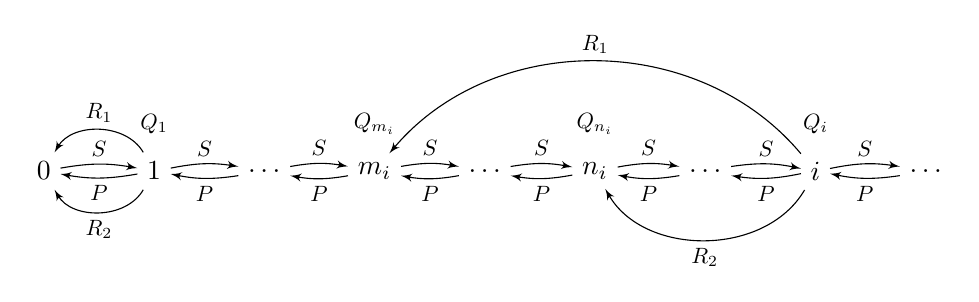
\begin{tikzpicture}[execute at begin node=$, execute at end node=$,
label/.style={scale=0.8},
every path/.style={->,>=latex'},node distance = 1.4cm]
\node (0) {0};
\node[right of=0] (1) {1};
\node[right of=1] (2) {\dots};
\node[right of=2] (3) {m_i};
\node[right of=3] (4) {\dots};
\node[right of=4] (5) {n_i};
\node[right of=5] (6) {\dots};
\node[right of=6] (7) {i};
\node[right of=7] (8) {\dots};


\node[node distance = 0.6cm,above of=1,label]     {Q_1};
\node[node distance = 0.6cm,above of=3,label]     {Q_{m_i}};
\node[node distance = 0.6cm,above of=5,label]     {Q_{n_i}};
\node[node distance = 0.6cm,above of=7,label]     {Q_i};


\foreach \x in {0,...,7}{
\pgfmathtruncatemacro{\xn}{\x+1}
\path (\xn) edge[bend left=10] node[below,label] {P} (\x);
\path (\x) edge[bend left=10] node[above,label] {S} (\xn);
}

\path (1) edge[bend right=60] node[above,label] {R_1} (0);
\path (1) edge[bend left=60] node[below,label] {R_2} (0);

\path (7) edge[bend right=50] node[above,label] {R_1} (3);
\path (7) edge[bend left=60] node[below,label] {R_2} (5);


\end{tikzpicture}
	\end{figure}
	We have $0\in E^I$, all other numbers are in $D^I$, and all numbers are in $G^I$.
	
	Here is the more formal definition of our model $I=(\N,\cdot^I,\omega)$.
	\begin{align*}
		  P^I&=\{(i+1,i)\mid i\in\N\}              & R_1^I&=\{(i,m_i)\mid i\in\N\} & R_2^I&=\{(i,n_i)\mid i\in\N\} \\
		  %Q^I&=\{ i\in\N\setminus\{0\}\mid Q=Q_i\} &  D^I&=\N\setminus\{0\}         & E^I&=\{0\}                            \\
		  S^I&=\{(i,i+1)\mid i\in\N\} &  D^I&=\{(i,i)\mid i\in\N^+\}         & E^I&=\{(0,0)\}                            \\
		  Q^I&=\{(i,i)\mid i\in\N, Q=Q_i\} \makebox[1mm]{\hspace{3cm}\text{for every $Q\in\autStates$}}& && \false^I&=\bot \\
		  G^I&=\N
	\end{align*}
	\begin{align*}
		  & a^I=0 &   & a_0^I=0 &   & b_0^I=0 
	\end{align*}
	Since there are no free variables in $\Gamma_M$ we can just set $\omega(x)=0$ for every $x\in\VarP$. It is easy to see that $I$ is indeed a model of $\Gamma_M$.
\end{proof}

We proof the other direction by induction on the length of the computation. But to be able to use the induction hypothesis we need a slightly more general statement (this is why we defined $\conGM$ and not just $\Gamma_M$ right away).
\begin{claim}\label{cla.18}
	Let $C=\langle Q,m,n\rangle$ be a configuration of $M$. If a final configuration (i.e. a configuration $\langle Q_f,\widehat{m},\widehat{n}\rangle$ for some $\widehat{m},\widehat{n}\in\N$) is reachable from $C$ then $\Gamma_C\cup\conGM\PModels\false$.
\end{claim}
\begin{proof} By induction on the length $i$ of the computation.
	
	Induction Base: $i=0$\\
	Since a final configuration is reachable in 0 steps $C$ must be this final configuration. So $C=\langle Q_f,m,n\rangle$ for some $m,n\in\N$. Hence, $Q_f(a)$ is in $\Gamma_C$ for some $a\in\VarP$ and $\forall\alpha(Q_f(\alpha)\to\false)$ is in $\conGM$, we can easily deduce false.
	\begin{figure}[H]
		\centering
		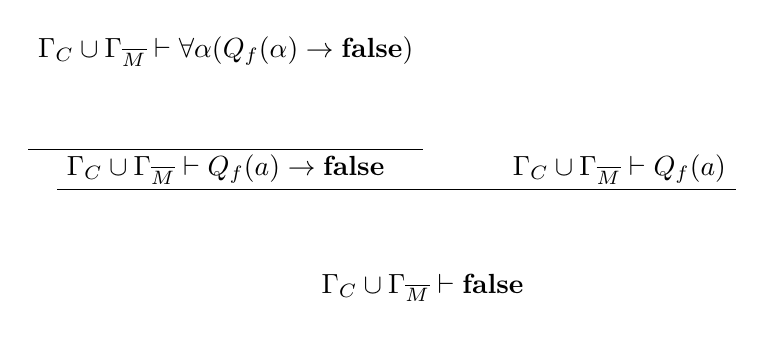
\begin{tikzpicture}[grow=up,
execute at begin node=$, execute at end node=$,
every node/.style={opacity=1},
every child/.style={edge from parent/.style={opacity=0}}]
\def\dist{0.6cm}
\node(e) {\Gamma_C\cup\conGM\vdash \false} [sibling distance=2*\dist+3.8cm] 
	child {node(1) {\Gamma_C\cup\conGM\vdash Q_f(a)}}
	child {node(2) {\Gamma_C\cup\conGM\vdash Q_f(a)\to\false}
		child {node(21) {\Gamma_C\cup\conGM\vdash\forall\alpha(Q_f(\alpha)\to\false)}}};


%tikz did not want to do this in the loop no idea why
%\coordinate(c1222) at (1222);
%\getwidthofnode{\sright}{12221}
%\draw (c1222)+(-\sright/2,+0.25) -- +(\sright/2,+0.25);

%set of all positions in the tree
\def\nodes{,1,2,11,12,21}
\def\identifier{0}
\foreach \x in \nodes{
\ifnodedefined{\x}{
	\coordinate(c\x) at (\x);
	\coordinate(\identifier.\x) at (0,0);
}{}
}

%draw lines for each node with 2 children (add parents with 2 children)
\foreach \x in \nodes{
\ifnodedefined{\identifier.\x1}{
	%calculate with of line
	\getwidthofnode{\sright}{\x1}
	%if there is a right child draw wide line
	\ifnodedefined{\identifier.\x2}{
		\getwidthofnode{\sleft}{\x2}
		%draw line
		\draw[shorten <=-\sright/2, shorten >=-\sleft/2] ([yshift=-0.25cm]c\x1) -- ([yshift=-0.25cm]c\x2);
	} %else only one child
	{
		\getwidthofnode{\sleft}{\x}
		%get widht corresponding to the widht of the bigger node
		\pgfmathsetlength{\sright}{max(\sright,\sleft)}
		%draw line
		\draw (c\x)+(-\sright/2,+0.25) -- +(\sright/2,+0.25);
	}
}{}
}
\end{tikzpicture}
	\end{figure}
	 
	Induction Step: $i= i'+1$\\
	Since $I\models\false$ holds trivially if $I$ interprets \false{} with $\top$ we only need to consider models of $\Gamma_C\cup\conGM$ that interpret \false{} with $\bot$ (note that there are no such models if $M$ terminates which is exactly what we want to proof). As result of this observation we can use the $\exists$-Introduction rule.
	
	From the fact that a final configuration is reachable from $C$ in $i$ steps we can deduce that there exists a configuration $D=\langle \widehat{Q}, \widehat{m}, \widehat{n}\rangle$ such that $C\Rightarrow_M^r D$ for some $r\in\mathcal{R}_\autStates$ and a final configuration is reachable from $D$ in $i'$ steps. We also know that $C=\langle Q,m,n\rangle$ for some $Q\in\autStates\setminus\{Q_f\}$ and some $m,n\in\N$.
	The set $\Gamma_C$ contains the formulas: 
	\begin{enumerate}[label=]%TODO is this a good idea?
		\item $R_1(a,a_0)$, $P(a_{i-1},a_i)$, $G(a_{i-1})$, and $D(a_{i-1})$ for $i\in\{1,\dots,m\}$,
		\item $R_2(a,b_0)$, $P(b_{i-1},b_i)$, $G(b_{i-1})$, and $D(b_{i-1})$ for $i\in\{1,\dots,n\}$,
		\item $Q(a)$, $E(a_m)$, $E(b_n)$, $G(a)$, $G(a_m)$, and $G(b_n)$.
	\end{enumerate}
	And $\Gamma_D$ contains the formulas:
	\begin{enumerate}[label=]
		\item $R_1(\widehat{a},\widehat{a}_0)$, $P(\widehat{a}_{i-1},\widehat{a}_i)$, $G(\widehat{a}_{i-1})$, and $D(\widehat{a}_{i-1})$ for $i\in\{1,\dots,\widehat{m}\}$,
		\item $R_2(\widehat{a},\widehat{b}_0)$, $P(\widehat{b}_{i-1},\widehat{b}_i)$, $G(\widehat{b}_{i-1})$, and $D(\widehat{b}_{i-1})$ for $i\in\{1,\dots,\widehat{n}\}$,
		\item $\widehat{Q}(\widehat{a})$, $E({\widehat{a}}_{\widehat{m}})$, $E({\widehat{b}}_{\widehat{n}})$, $G(\widehat{a})$, $G({\widehat{a}}_{\widehat{m}})$, and $G({\widehat{b}}_{\widehat{n}})$.
	\end{enumerate}
	The basic idea is to deduce $\Gamma_D$ from $\Gamma_C\cup\conGM$ and then apply the induction hypothesis to $\Gamma_D\cup\conGM$. 
	
	\begin{figure}[H]
		\centering
		
\begin{tikzpicture}[grow=up,level distance=0.5cm,
execute at begin node=$, execute at end node=$,
every node/.style={opacity=1},
every child/.style={edge from parent/.style={opacity=0}}]
\def\dist{0.6cm}
\node(e) {\Gamma_C\cup\conGM\vdashf \falses} [sibling distance=2*\dist+2.4cm] 
	child {node(1) {\Gamma_C\cup\conGM\vdashf \Gamma_D}}
	child {node(2) {\Gamma_C\cup\conGM\cup \Gamma_D\vdashf\falses}
		child {node(21) {IH}}};


%tikz did not want to do this in the loop no idea why
%\coordinate(c1222) at (1222);
%\getwidthofnode{\sright}{12221}
%\draw (c1222)+(-\sright/2,+0.25) -- +(\sright/2,+0.25);

%set of all positions in the tree
\def\nodes{,1,2,11,12,21}
%the yshift does not work on nodes so we create a coordinate for every node
\foreach \x in \nodes{
\ifnodedefined{\x}{
	\coordinate(c\x) at (\x);
}{}
}

%draw lines for each node with 2 children (add parents with 2 children)
\foreach \x in \nodes{
\ifnodedefined{\x1}{
	%calculate with of line
	\getwidthofnode{\sright}{\x1}
	%if there is a right child draw wide line
	\ifnodedefined{\x2}{
		\getwidthofnode{\sleft}{\x2}
		%draw line
		\draw[shorten <=-\sright/2, shorten >=-\sleft/2] ([yshift=-0.25cm]c\x1) -- ([yshift=-0.25cm]c\x2);
	} %else only one child
	{
		\getwidthofnode{\sleft}{\x}
		%get widht corresponding to the widht of the bigger node
		\pgfmathsetlength{\sright}{max(\sright,\sleft)}
		%draw line
		\draw (c\x)+(-\sright/2,+0.25) -- +(\sright/2,+0.25);
	}
}{}
}
\end{tikzpicture}
	\end{figure}
	
	We achieve this by looking at the four possible cases for the type of the rule $r$. We will only consider the cases $r=+(1,Q')$ and $r=-(1,Q_1,Q_2)$, because the two remaining cases $r=+(2,Q')$ and $r=-(2,Q_1,Q_2)$ follow by exchanging the roles of register 1 and register 2 in the first two cases.
	
	First we need a new free variable representing the configuration $D$. Also the value in register 2 does not change, because in both cases we are only concerned with register 1.
	For the succeeding tableau proofs we will abbreviate \false{} by \falses{} and we will drop $\Gamma_C\cup\conGM$ and only write new formulas on the left side of $\PModelsf$.
	
	We first introduce a new variable representing the new configuration $D$ (let $b\in \VarP\setminus\text{FV}(\Gamma_C)$, note that $\FV(\conGM)=\emptyset$).
	
	\begin{figure}[H]
		\centering
		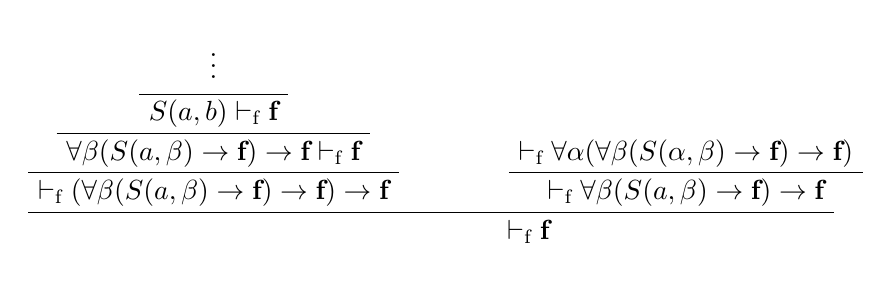
\begin{tikzpicture}[grow=up,level distance=0.5cm,
execute at begin node=$, execute at end node=$,
every node/.style={opacity=1},
every child/.style={edge from parent/.style={opacity=0}}]
\node(e) {\PModelsf \falses} [sibling distance=8cm] 
	child [sibling distance=4cm] {node(1) {\PModelsf\forall\beta(S(a,\beta)\to\falses)\to\falses} 
		child {node(11) {\PModelsf\forall\alpha(\forall\beta(S(\alpha,\beta)\to\falses)\to\falses)}}}
	child {node(2) {\PModelsf(\forall\beta(S(a,\beta)\to\falses)\to\falses)\to\falses}
		child {node(21) {\forall\beta(S(a,\beta)\to\falses)\to\falses\PModelsf\falses}
			child {node(211) {S(a,b)\PModelsf\falses}
				child {node[label={[yshift=-0.3cm]above:\vdots}](2111) {}}}}};

%set of all positions in the tree
\def\nodes{,1,2,11,21,211,2111}
%the yshift does not work on nodes so we create a coordinate for every node
\foreach \x in \nodes{
\ifnodedefined{\x}{
	\coordinate(c\x) at (\x);
	\coordinate(1.\x) at (0,0); %we need this because defined nodes are not fergotten between tikz pictures
}{}
}

%draw lines for each node with 2 children (add parents with 2 children)
\foreach \x in \nodes{
\ifnodedefined{1.\x1}{
	%calculate with of line
	\getwidthofnode{\sright}{\x1}
	%if there is a right child draw wide line
	\ifnodedefined{1.\x2}{
		\getwidthofnode{\sleft}{\x2}
		%draw line
		\draw[shorten <=-\sright/2, shorten >=-\sleft/2] ([yshift=-0.25cm]c\x1) -- ([yshift=-0.25cm]c\x2);
	} %else only one child
	{
		\getwidthofnode{\sleft}{\x}
		%get widht corresponding to the widht of the bigger node
		\pgfmathsetlength{\sright}{max(\sright,\sleft)}
		%draw line
		\draw (c\x)+(-\sright/2,+0.25) -- +(\sright/2,+0.25);
	}
}{}
}

\end{tikzpicture}
	\end{figure}
	
	For the new variable $b$ we have to deduce $G(b)$.
	
	\begin{figure}[H]
		\centering
		\begin{tikzpicture}[grow=up,
execute at begin node=$, execute at end node=$,
every node/.style={opacity=1},
every child/.style={edge from parent/.style={opacity=0}}]
\def\dist{0.7cm}
\node(e) {\PModelsf \falses} [sibling distance=2*\dist+4.4cm] 
	child {node(1) {\PModelsf G(b)} [sibling distance=\dist+2.9cm]
		child {node(11) {\PModelsf S(a,b)}}
		child {node(12) {\PModelsf S(a,b)\to G(b)}
			child {node(121) {\PModelsf \forall\alpha\beta(S(\alpha,\beta)\to G(\beta))}}}
	}
	child {node(2) {\PModelsf G(b)\to\falses}
		child {node(21) {G(b)\PModelsf\falses}
			child {node[label={[yshift=-0.3cm]above:\vdots}](211) {}}}};



%set of all positions in the tree
\def\nodes{,1,2,21,211,11,12,121}
\def\identifier{10}
\foreach \x in \nodes{
\ifnodedefined{\x}{
	\coordinate(c\x) at (\x);
	\coordinate(\identifier.\x) at (0,0);
}{}
}

%draw lines for each node with 2 children (add parents with 2 children)
\foreach \x in \nodes{
\ifnodedefined{\identifier.\x1}{
	%calculate with of line
	\getwidthofnode{\sright}{\x1}
	%if there is a right child draw wide line
	\ifnodedefined{\identifier.\x2}{
		\getwidthofnode{\sleft}{\x2}
		%draw line
		\draw[shorten <=-\sright/2, shorten >=-\sleft/2] ([yshift=-0.25cm]c\x1) -- ([yshift=-0.25cm]c\x2);
	} %else only one child
	{
		\getwidthofnode{\sleft}{\x}
		%get widht corresponding to the widht of the bigger node
		\pgfmathsetlength{\sright}{max(\sright,\sleft)}
		%draw line
		\draw (c\x)+(-\sright/2,+0.25) -- +(\sright/2,+0.25);
	}
}{}
}
\end{tikzpicture}
	\end{figure}
	
	Since register 2 should not change we need $R_2(b,b_0)$. Again we will just drop $S(a,b)$ on the left side for comprehensibility.
		
	\begin{figure}[H]
		\centering
		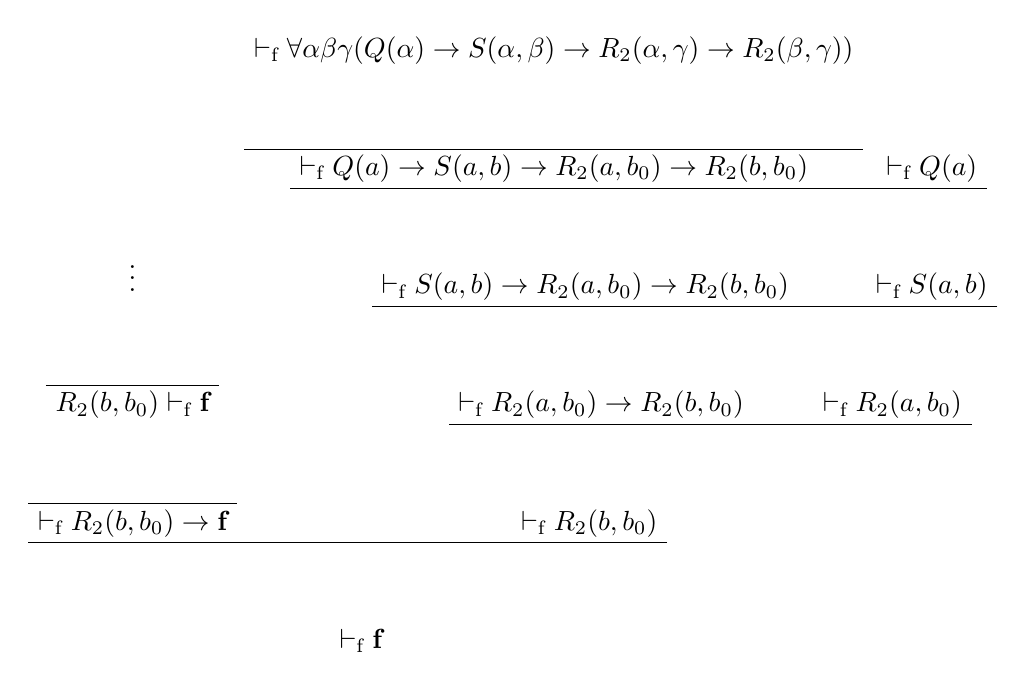
\begin{tikzpicture}[grow=up,
execute at begin node=$, execute at end node=$,
every node/.style={opacity=1},
every child/.style={edge from parent/.style={opacity=0}}]
\def\dist{0.4cm}
\node(e) {\PModelsf \falses} [sibling distance=2*\dist+5cm] 
	child {node(1) {\PModelsf R_2(b,b_0)} [sibling distance=\dist+3.3cm]
		child[xshift=2cm] {node(11) {\PModelsf R_2(a,b_0)}}
		child[xshift=2cm] {node(12) {\PModelsf R_2(a,b_0)\to R_2(b,b_0)} [sibling distance=\dist+4cm]
			child[xshift=2cm] {node(121) {\PModelsf S(a,b)}}
			child[xshift=2cm] {node(122) {\PModelsf S(a,b)\to R_2(a,b_0)\to R_2(b,b_0)} [sibling distance=\dist+4.4cm]
				child[xshift=2cm] {node(1221) {\PModelsf Q(a)}}
				child[xshift=2cm] {node(1222) {\PModelsf Q(a)\to S(a,b)\to R_2(a,b_0)\to R_2(b,b_0)}
					child {node(12221) {\PModelsf\forall\alpha\beta\gamma(Q(\alpha)\to S(\alpha,\beta)\to R_2(\alpha,\gamma)\to R_2(\beta,\gamma))}}}}}}
	child {node(2) {\PModelsf R_2(b,b_0)\to\falses}
		child {node(21) {R_2(b,b_0)\PModelsf\falses}
			child {node[label={[yshift=-0.3cm]above:\vdots}](211) {}}}};


%set of all positions in the tree
\def\nodes{,1,2,11,12,21,121,122,1221,1222,12221,211}
\def\identifier{6}
\foreach \x in \nodes{
\ifnodedefined{\x}{
	\coordinate(c\x) at (\x);
	\coordinate(\identifier.\x) at (0,0);
}{}
}

%draw lines for each node with 2 children (add parents with 2 children)
\foreach \x in \nodes{
\ifnodedefined{\identifier.\x1}{
	%calculate with of line
	\getwidthofnode{\sright}{\x1}
	%if there is a right child draw wide line
	\ifnodedefined{\identifier.\x2}{
		\getwidthofnode{\sleft}{\x2}
		%draw line
		\draw[shorten <=-\sright/2, shorten >=-\sleft/2] ([yshift=-0.25cm]c\x1) -- ([yshift=-0.25cm]c\x2);
	} %else only one child
	{
		\getwidthofnode{\sleft}{\x}
		%get widht corresponding to the widht of the bigger node
		\pgfmathsetlength{\sright}{max(\sright,\sleft)}
		%draw line
		\draw (c\x)+(-\sright/2,+0.25) -- +(\sright/2,+0.25);
	}
}{}
}
\end{tikzpicture}
	\end{figure}
	
	For the case that $\boldsymbol{r=+(1,Q')}$, we have that $\widehat{Q}=Q'$, $\widehat{m}=m+1$, and $\widehat{n}=n$. So we need to increment register 1 and ensure that the state of $b$ is $Q'$.
	\begin{figure}[H]
		\centering
		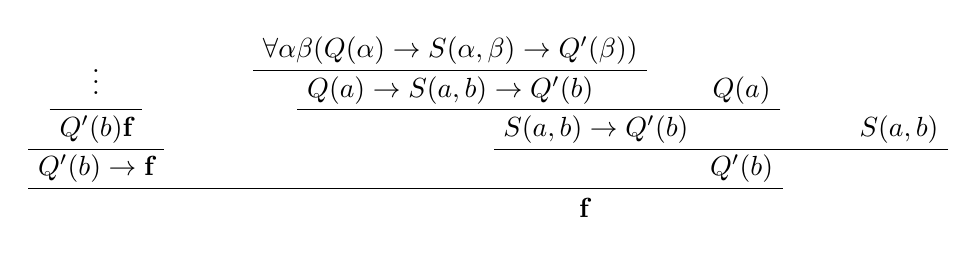
\begin{tikzpicture}[grow=up,level distance=0.5cm,
execute at begin node=$, execute at end node=$,
every node/.style={opacity=1},
every child/.style={edge from parent/.style={opacity=0}}]
\node(e) {\vdashf \falses} [sibling distance=12.4cm] 
	child [sibling distance=4cm] {node(1) {\vdashf Q'(b)} 
		child {node(11) {\vdashf S(a,b)} }
		child [sibling distance=3.7cm] {node(12) {\vdashf S(a,b)\to Q'(b)} 
			child {node(121) {\vdashf Q(a)} }
			child {node(122) {\vdashf Q(a)\to S(a,b)\to Q'(b)} 
				child {node(1221) {\vdashf\forall\alpha\beta(Q(\alpha)\to S(\alpha,\beta)\to Q'(\beta))} }}}}
	child {node(2) {\vdashf Q'(b)\to\falses} 
		child {node(21) {Q'(b)\vdashf\falses} 
			child {node[label={[yshift=-0.3cm]above:\vdots}](211) {}}}};

%set of all positions in the tree
\def\nodes{,1,2,11,12,21,121,122,1221,211}
%the yshift does not work on nodes so we create a coordinate for every node
\foreach \x in \nodes{
\ifnodedefined{\x}{
	\coordinate(c\x) at (\x);
	\coordinate(3.\x) at (0,0);
}{}
}

%draw lines for each node with 2 children (add parents with 2 children)
\foreach \x in \nodes{
\ifnodedefined{3.\x1}{
	%calculate with of line
	\getwidthofnode{\sright}{\x1}
	%if there is a right child draw wide line
	\ifnodedefined{3.\x2}{
		\getwidthofnode{\sleft}{\x2}
		%draw line
		\draw[shorten <=-\sright/2, shorten >=-\sleft/2] ([yshift=-0.25cm]c\x1) -- ([yshift=-0.25cm]c\x2);
	} %else only one child
	{
		\getwidthofnode{\sleft}{\x}
		%get widht corresponding to the widht of the bigger node
		\pgfmathsetlength{\sright}{max(\sright,\sleft)}
		%draw line
		\draw (c\x)+(-\sright/2,+0.25) -- +(\sright/2,+0.25);
	}
}{}
}
\end{tikzpicture}
	\end{figure}
	
	To increment register 1 we need a new free variable as anchor for register 1 (let $d\in\VarP\setminus\text{FV}(\Gamma_C)$ and $d\neq b$).
	
	\begin{figure}[H]
		\centering
		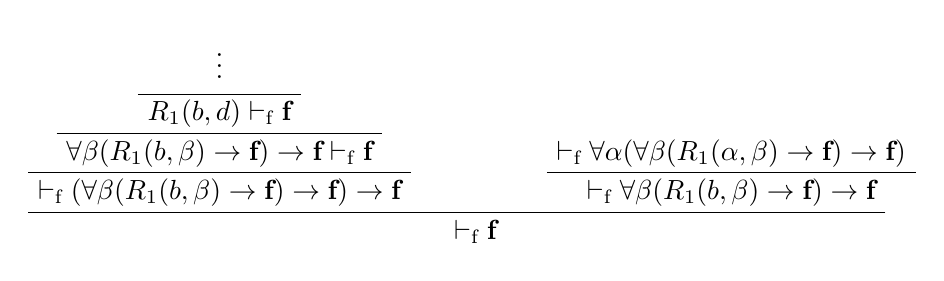
\begin{tikzpicture}[grow=up,level distance=0.5cm,
execute at begin node=$, execute at end node=$,
every node/.style={opacity=1},
every child/.style={edge from parent/.style={opacity=0}}]
\node(e) {\PModelsf\falses} [sibling distance=6.5cm]
	child {node(1) {\PModelsf\forall\beta(R_1(b,\beta)\to\falses)\to\falses} [sibling distance=4cm]
		child {node(11) {\PModelsf\forall\alpha(\forall\beta(R_1(\alpha,\beta)\to\falses)\to\falses)}}}
	child {node(2) {\PModelsf(\forall\beta(R_1(b,\beta)\to\falses)\to\falses)\to\falses}
		child {node(21) {\forall\beta(R_1(b,\beta)\to\falses)\to\falses\PModelsf\falses}
			child {node(211) {R_1(b,d)\PModelsf\falses}
				child {node[label={[yshift=-0.3cm]above:\vdots}](2111) {}}}}};

%set of all positions in the tree
\def\nodes{,1,2,11,21,211,2111}
%the yshift does not work on nodes so we create a coordinate for every node
\foreach \x in \nodes{
\ifnodedefined{\x}{
	\coordinate(c\x) at (\x);
	\coordinate(2.\x) at (0,0);
}{}
}

%draw lines for each node with 2 children (add parents with 2 children)
\foreach \x in \nodes{
\ifnodedefined{2.\x1}{
	%calculate with of line
	\getwidthofnode{\sright}{\x1}
	%if there is a right child draw wide line
	\ifnodedefined{2.\x2}{
		\getwidthofnode{\sleft}{\x2}
		%draw line
		\draw[shorten <=-\sright/2, shorten >=-\sleft/2] ([yshift=-0.25cm]c\x1) -- ([yshift=-0.25cm]c\x2);
	} %else only one child
	{
		\getwidthofnode{\sleft}{\x}
		%get widht corresponding to the widht of the bigger node
		\pgfmathsetlength{\sright}{max(\sright,\sleft)}
		%draw line
		\draw (c\x)+(-\sright/2,+0.25) -- +(\sright/2,+0.25);
	}
}{}
}

\end{tikzpicture}
	\end{figure}
	
	Now we need to connect $d$ with $a_0$ (the anchor of $a$ for register 1).
	
	\begin{figure}[H]
		\centering
		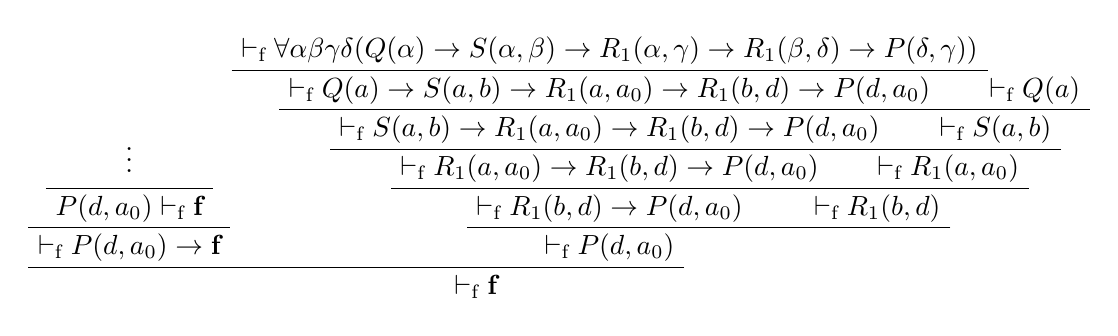
\begin{tikzpicture}[grow=up,level distance=0.5cm,
execute at begin node=$, execute at end node=$,
every node/.style={opacity=1},
every child/.style={edge from parent/.style={opacity=0}}]
\def\dist{0.4cm}
\node(e) {\PModelsf \falses} [sibling distance=2*\dist+8cm] 
	child [sibling distance=\dist+3cm] {node(1) {\PModelsf P(d,a_0)} 
		child {node(11) {\PModelsf R_1(b,d)} }
		child [sibling distance=\dist+3.9cm] {node(12) {\PModelsf R_1(b,d)\to P(d,a_0)} 
			child {node(121) {\PModelsf R_1(a,a_0)} }
			child [sibling distance=\dist+4.5cm] {node(122) {\PModelsf R_1(a,a_0)\to R_1(b,d)\to P(d,a_0)} 
				child {node(1221) {\PModelsf S(a,b)} }
				child [sibling distance=\dist+5cm] {node(1222) {\PModelsf S(a,b)\to R_1(a,a_0)\to R_1(b,d)\to P(d,a_0)}
					child {node(12221) {\PModelsf Q(a)} }
					child {node(12222) {\PModelsf Q(a)\to S(a,b)\to R_1(a,a_0)\to R_1(b,d)\to P(d,a_0)}
						child {node(122221) {\PModelsf \forall\alpha\beta\gamma\delta(Q(\alpha)\to S(\alpha,\beta)\to R_1(\alpha,\gamma)\to R_1(\beta,\delta)\to P(\delta,\gamma))}}}
					child {}}
				child {}}
			child {}}
		child {}}
				%child {node(1221) {\PModelsf\forall\alpha\beta(Q(\alpha)\to S(\alpha,\beta)\to Q'(\beta))} }}}}
	child {node(2) {\PModelsf P(d,a_0)\to\falses} 
		child {node(21) {P(d,a_0)\PModelsf\falses} 
			child {node[label={[yshift=-0.3cm]above:\vdots}](211) {}}}};

%set of all positions in the tree
\def\nodes{,1,2,11,12,21,121,122,1221,1222,12221,12222,122221,211}
%the yshift does not work on nodes so we create a coordinate for every node
\foreach \x in \nodes{
\ifnodedefined{\x}{
	\coordinate(c\x) at (\x);
	\coordinate(4.\x) at (0,0);
}{}
}

%draw lines for each node with 2 children (add parents with 2 children)
\foreach \x in \nodes{
\ifnodedefined{4.\x1}{
	%calculate with of line
	\getwidthofnode{\sright}{\x1}
	%if there is a right child draw wide line
	\ifnodedefined{4.\x2}{
		\getwidthofnode{\sleft}{\x2}
		%draw line
		\draw[shorten <=-\sright/2, shorten >=-\sleft/2] ([yshift=-0.25cm]c\x1) -- ([yshift=-0.25cm]c\x2);
	} %else only one child
	{
		\getwidthofnode{\sleft}{\x}
		%get widht corresponding to the widht of the bigger node
		\pgfmathsetlength{\sright}{max(\sright,\sleft)}
		%draw line
		\draw (c\x)+(-\sright/2,+0.25) -- +(\sright/2,+0.25);
	}
}{}
}
\end{tikzpicture}
	\end{figure}
	
	We have to make sure that we do not get an artificial zero. We achieve this by deducing $D(d)$.
	
	\begin{figure}[H]
		\centering
		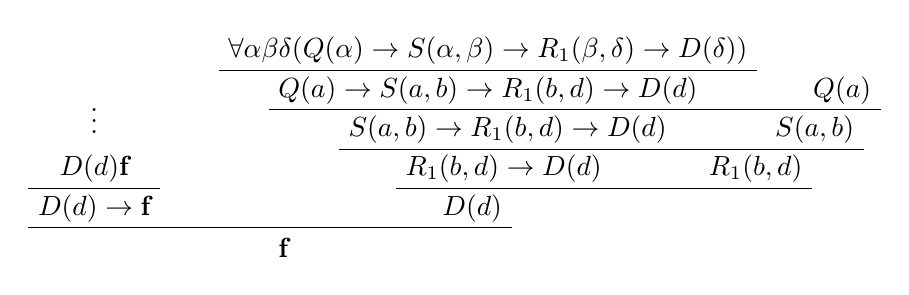
\begin{tikzpicture}[grow=up,level distance=0.5cm,
execute at begin node=$, execute at end node=$,
every node/.style={opacity=1},
every child/.style={edge from parent/.style={opacity=0}}]
\def\dist{0.4cm}
\node(e) {\vdashf \falses} [sibling distance=2*\dist+4cm] 
	child {node(1) {\vdashf D(d)} [sibling distance=\dist+2.8cm]
		child[xshift=2cm] {node(11) {\vdashf R_1(b,d)}}
		child[xshift=2cm] {node(12) {\vdashf R_1(b,d)\to D(d)} [sibling distance=\dist+3.5cm]
			child[xshift=2cm] {node(121) {\vdashf S(a,b)}}
			child[xshift=2cm] {node(122) {\vdashf S(a,b)\to R_1(b,d)\to D(d)} [sibling distance=\dist+4.1cm]
				child[xshift=2cm] {node(1221) {\vdashf Q(a)}}
				child[xshift=2cm] {node(1222) {\vdashf Q(a)\to S(a,b)\to R_1(b,d)\to D(d)}
					child {node(12221) {\vdashf\forall\alpha\beta\delta(Q(\alpha)\to S(\alpha,\beta)\to R_1(\beta,\delta)\to D(\delta))}}}}}}
	child {node(2) {\vdashf D(d)\to\falses}
		child {node(21) {D(d)\vdashf\falses}
			child {node[label={[yshift=-0.3cm]above:\vdots}](211) {}}}};



%set of all positions in the tree
\def\nodes{,1,2,11,12,21,121,122,1221,1222,12221}
%the yshift does not work on nodes so we create a coordinate for every node
\foreach \x in \nodes{
\ifnodedefined{\x}{
	\coordinate(c\x) at (\x);
	\coordinate(5.\x) at (0,0);
}{}
}

%draw lines for each node with 2 children (add parents with 2 children)
\foreach \x in \nodes{
\ifnodedefined{5.\x1}{
	%calculate with of line
	\getwidthofnode{\sright}{\x1}
	%if there is a right child draw wide line
	\ifnodedefined{5.\x2}{
		\getwidthofnode{\sleft}{\x2}
		%draw line
		\draw[shorten <=-\sright/2, shorten >=-\sleft/2] ([yshift=-0.25cm]c\x1) -- ([yshift=-0.25cm]c\x2);
	} %else only one child
	{
		\getwidthofnode{\sleft}{\x}
		%get widht corresponding to the widht of the bigger node
		\pgfmathsetlength{\sright}{max(\sright,\sleft)}
		%draw line
		\draw (c\x)+(-\sright/2,+0.25) -- +(\sright/2,+0.25);
	}
}{}
}
\end{tikzpicture}
	\end{figure}
	
	Now we can easily deduce $G(d)$.
	
	\begin{figure}[H]
		\centering
		\begin{tikzpicture}[grow=up,
execute at begin node=$, execute at end node=$,
every node/.style={opacity=1},
every child/.style={edge from parent/.style={opacity=0}}]
\def\dist{0.7cm}
\node(e) {\PModelsf \falses} [sibling distance=2*\dist+4.4cm] 
	child {node(1) {\PModelsf G(d)} [sibling distance=\dist+2.9cm]
		child {node(11) {\PModelsf D(d)}}
		child {node(12) {\PModelsf D(d)\to G(d)}
			child {node(121) {\PModelsf \forall\alpha(D(\alpha)\to G(\alpha))}}}
	}
	child {node(2) {\PModelsf G(d)\to\falses}
		child {node(21) {G(d)\PModelsf\falses}
			child {node[label={[yshift=-0.3cm]above:\vdots}](211) {}}}};



%set of all positions in the tree
\def\nodes{,1,2,21,11,12,121}
\def\identifier{10}
\foreach \x in \nodes{
\ifnodedefined{\x}{
	\coordinate(c\x) at (\x);
	\coordinate(\identifier.\x) at (0,0);
}{}
}

%draw lines for each node with 2 children (add parents with 2 children)
\foreach \x in \nodes{
\ifnodedefined{\identifier.\x1}{
	%calculate with of line
	\getwidthofnode{\sright}{\x1}
	%if there is a right child draw wide line
	\ifnodedefined{\identifier.\x2}{
		\getwidthofnode{\sleft}{\x2}
		%draw line
		\draw[shorten <=-\sright/2, shorten >=-\sleft/2] ([yshift=-0.25cm]c\x1) -- ([yshift=-0.25cm]c\x2);
	} %else only one child
	{
		\getwidthofnode{\sleft}{\x}
		%get widht corresponding to the widht of the bigger node
		\pgfmathsetlength{\sright}{max(\sright,\sleft)}
		%draw line
		\draw (c\x)+(-\sright/2,+0.25) -- +(\sright/2,+0.25);
	}
}{}
}
\end{tikzpicture}
	\end{figure}
	
	Now we already have deduced $\Gamma_D$, to see why define $\widehat{a}:=b$, $\widehat{b}_i:=b_i$ for $i\in\{0,\dots,n\}$, $\widehat{a}_0:=d$, and $\widehat{a}_{i+1}:=a_i$ for $i\in\{0,\dots,m\}$.
	Hence we can deduce \false{} by induction hypothesis.\\
	
	The other case, that $\boldsymbol{r=-(Q,1,Q_1,Q_2)}$, has to be split into two cases again. If $\boldsymbol{m=0}$ then $\widehat{Q}=Q_2$, $\widehat{m}=0$, and $\widehat{n}=n$. We only need to ensure that the successor state is $Q_2$ and that register 1 is still zero.
	
	\begin{figure}[H]
		\centering
		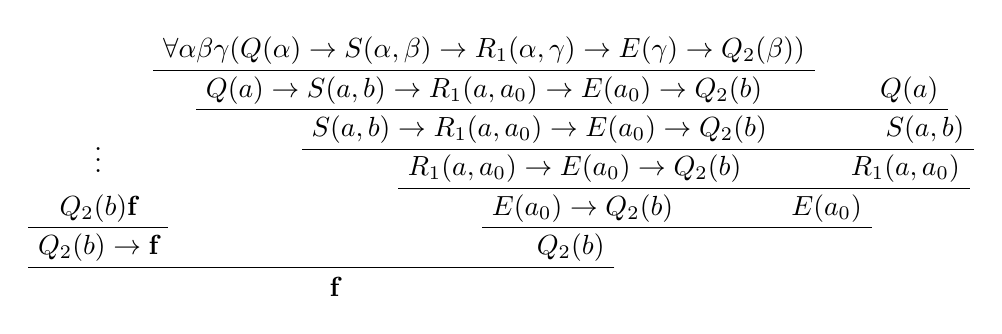
\begin{tikzpicture}[grow=up,level distance=0.5cm,
execute at begin node=$, execute at end node=$,
every node/.style={opacity=1},
every child/.style={edge from parent/.style={opacity=0}}]
\def\dist{0.4cm}
\node(e) {\vdashf \falses} [sibling distance=6cm] 
	child {node(1) {\vdashf Q_2(b)} [sibling distance=\dist+2.7cm]
		child[xshift=1.7cm] {node(11) {\vdashf E(a_0)}}
		child[xshift=1.7cm] {node(12) {\vdashf E(a_0)\to Q_2(b)} [sibling distance=\dist+3.8cm]
			child[xshift=2cm] {node(121) {\vdashf R_1(a,a_0)}}
			child[xshift=2cm] {node(122) {\vdashf R_1(a,a_0)\to E(a_0)\to Q_2(b)} [sibling distance=\dist+4.5cm]
				child[xshift=2cm] {node(1221) {\vdashf S(a,b)}}
				child[xshift=2cm] {node(1222) {\vdashf S(a,b)\to R_1(a,a_0)\to E(a_0)\to Q_2(b)} [sibling distance=\dist+5cm]
					child[xshift=2cm] {node(12221) {\vdashf Q(a)}}
					child[xshift=2cm] {node(12222) {\vdashf Q(a)\to S(a,b)\to R_1(a,a_0)\to E(a_0)\to Q_2(b)}
						child {node(122221) {\vdashf\forall\alpha\beta\gamma(Q(\alpha)\to S(\alpha,\beta)\to R_1(\alpha,\gamma)\to E(\gamma)\to Q_2(\beta))}}}}}}}
	child {node(2) {\vdashf Q_2(b)\to\falses}
		child {node(21) {Q_2(b)\vdashf\falses}
			child {node[label={[yshift=-0.3cm]above:\vdots}](211) {}}}};


%set of all positions in the tree
\def\nodes{,1,2,11,12,21,121,122,1221,1222,12222,12221,12222,122221}
%the yshift does not work on nodes so we create a coordinate for every node
\foreach \x in \nodes{
\ifnodedefined{\x}{
	\coordinate(c\x) at (\x);
	\coordinate(7.\x) at (0,0);
}{}
}

%draw lines for each node with 2 children (add parents with 2 children)
\foreach \x in \nodes{
\ifnodedefined{7.\x1}{
	%calculate with of line
	\getwidthofnode{\sright}{\x1}
	%if there is a right child draw wide line
	\ifnodedefined{7.\x2}{
		\getwidthofnode{\sleft}{\x2}
		%draw line
		\draw[shorten <=-\sright/2, shorten >=-\sleft/2] ([yshift=-0.25cm]c\x1) -- ([yshift=-0.25cm]c\x2);
	} %else only one child
	{
		\getwidthofnode{\sleft}{\x}
		%get widht corresponding to the widht of the bigger node
		\pgfmathsetlength{\sright}{max(\sright,\sleft)}
		%draw line
		\draw (c\x)+(-\sright/2,+0.25) -- +(\sright/2,+0.25);
	}
}{}
}
\end{tikzpicture}
	\end{figure}
	
	Register 1 stays zero.
	
	\begin{figure}[H]
		\centering
		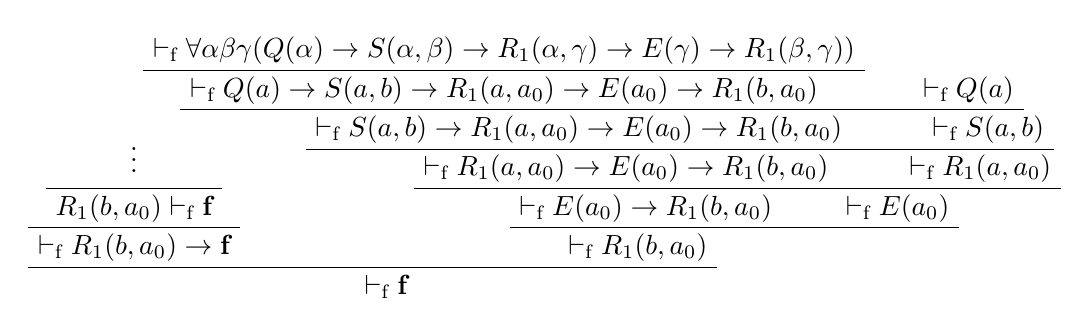
\begin{tikzpicture}[grow=up,level distance=0.5cm,
execute at begin node=$, execute at end node=$,
every node/.style={opacity=1},
every child/.style={edge from parent/.style={opacity=0}}]
\node(e) {\PModelsf \falses} [sibling distance=6.4cm] 
	child {node(1) {\PModelsf R_1(b,a_0)} [sibling distance=3.2cm]
		child[xshift=1.7cm] {node(11) {\PModelsf E(a_0)}}
		child[xshift=1.7cm] {node(12) {\PModelsf E(a_0)\to R_1(b,a_0)} [sibling distance=4.5cm]
			child[xshift=2cm] {node(121) {\PModelsf R_1(a,a_0)}}
			child[xshift=2cm] {node(122) {\PModelsf R_1(a,a_0)\to E(a_0)\to R_1(b,a_0)} [sibling distance=5.2cm]
				child[xshift=2cm] {node(1221) {\PModelsf S(a,b)}}
				child[xshift=2cm] {node(1222) {\PModelsf S(a,b)\to R_1(a,a_0)\to E(a_0)\to R_1(b,a_0)} [sibling distance=5.9cm]
					child[xshift=2cm] {node(12221) {\PModelsf Q(a)}}
					child[xshift=2cm] {node(12222) {\PModelsf Q(a)\to S(a,b)\to R_1(a,a_0)\to E(a_0)\to R_1(b,a_0)}
						child {node(122221) {\PModelsf\forall\alpha\beta\gamma(Q(\alpha)\to S(\alpha,\beta)\to R_1(\alpha,\gamma)\to E(\gamma)\to R_1(\beta,\gamma))}}}}}}}
	child {node(2) {\PModelsf R_1(b,a_0)\to\falses}
		child {node(21) {R_1(b,a_0)\PModelsf\falses}
			child {node[label={[yshift=-0.3cm]above:\vdots}](211) {}}}};


%set of all positions in the tree
\def\nodes{,1,2,11,12,21,121,122,1221,1222,12222,12221,12222,122221,211}
\def\identifier{8}
\foreach \x in \nodes{
\ifnodedefined{\x}{
	\coordinate(c\x) at (\x);
	\coordinate(\identifier.\x) at (0,0);
}{}
}

%draw lines for each node with 2 children (add parents with 2 children)
\foreach \x in \nodes{
\ifnodedefined{\identifier.\x1}{
	%calculate with of line
	\getwidthofnode{\sright}{\x1}
	%if there is a right child draw wide line
	\ifnodedefined{\identifier.\x2}{
		\getwidthofnode{\sleft}{\x2}
		%draw line
		\draw[shorten <=-\sright/2, shorten >=-\sleft/2] ([yshift=-0.25cm]c\x1) -- ([yshift=-0.25cm]c\x2);
	} %else only one child
	{
		\getwidthofnode{\sleft}{\x}
		%get widht corresponding to the widht of the bigger node
		\pgfmathsetlength{\sright}{max(\sright,\sleft)}
		%draw line
		\draw (c\x)+(-\sright/2,+0.25) -- +(\sright/2,+0.25);
	}
}{}
}
\end{tikzpicture}
	\end{figure}
	
	If we define $\widehat{a}:=b$, $\widehat{b}_i:=b_i$ for $i\in\{0,\dots,n\}$, and $\widehat{a}_0:=a_0$ then it is clear that we have deduced all formulas required for $\Gamma_D$. So we can use the induction hypothesis to deduce \false{}.
	
	In the last case $\boldsymbol{m>0}$, so $\widehat{Q}=Q_1$, $\widehat{m}=m-1$, and $\widehat{n}=n$. First we ensure that $b$ is in state $Q_1$.
	
	\begin{figure}[H]
		\centering
		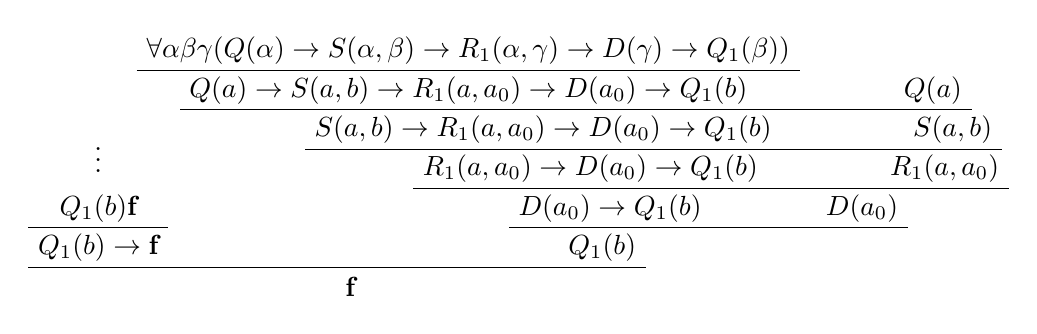
\begin{tikzpicture}[grow=up,level distance=0.5cm,
execute at begin node=$, execute at end node=$,
every node/.style={opacity=1},
every child/.style={edge from parent/.style={opacity=0}}]
\node(e) {\vdashf \falses} [sibling distance=6.4cm] 
	child {node(1) {\vdashf Q_1(b)} [sibling distance=3.2cm]
		child[xshift=1.7cm] {node(11) {\vdashf D(a_0)}}
		child[xshift=1.7cm] {node(12) {\vdashf D(a_0)\to Q_1(b)} [sibling distance=4.5cm]
			child[xshift=2cm] {node(121) {\vdashf R_1(a,a_0)}}
			child[xshift=2cm] {node(122) {\vdashf R_1(a,a_0)\to D(a_0)\to Q_1(b)} [sibling distance=5.2cm]
				child[xshift=2cm] {node(1221) {\vdashf S(a,b)}}
				child[xshift=2cm] {node(1222) {\vdashf S(a,b)\to R_1(a,a_0)\to D(a_0)\to Q_1(b)} [sibling distance=5.9cm]
					child[xshift=2cm] {node(12221) {\vdashf Q(a)}}
					child[xshift=2cm] {node(12222) {\vdashf Q(a)\to S(a,b)\to R_1(a,a_0)\to D(a_0)\to Q_1(b)}
						child {node(122221) {\vdashf\forall\alpha\beta\gamma(Q(\alpha)\to S(\alpha,\beta)\to R_1(\alpha,\gamma)\to D(\gamma)\to Q_1(\beta))}}}}}}}
	child {node(2) {\vdashf Q_1(b)\to\falses}
		child {node(21) {Q_1(b)\vdashf\falses}
			child {node[label={[yshift=-0.3cm]above:\vdots}](211) {}}}};



%set of all positions in the tree
\def\nodes{,1,2,11,12,21,121,122,1221,1222,12222,12221,12222,122221}
%the yshift does not work on nodes so we create a coordinate for every node
\foreach \x in \nodes{
\ifnodedefined{\x}{
	\coordinate(c\x) at (\x);
	\coordinate(9.\x) at (0,0);
}{}
}

%draw lines for each node with 2 children (add parents with 2 children)
\foreach \x in \nodes{
\ifnodedefined{9.\x1}{
	%calculate with of line
	\getwidthofnode{\sright}{\x1}
	%if there is a right child draw wide line
	\ifnodedefined{9.\x2}{
		\getwidthofnode{\sleft}{\x2}
		%draw line
		\draw[shorten <=-\sright/2, shorten >=-\sleft/2] ([yshift=-0.25cm]c\x1) -- ([yshift=-0.25cm]c\x2);
	} %else only one child
	{
		\getwidthofnode{\sleft}{\x}
		%get widht corresponding to the widht of the bigger node
		\pgfmathsetlength{\sright}{max(\sright,\sleft)}
		%draw line
		\draw (c\x)+(-\sright/2,+0.25) -- +(\sright/2,+0.25);
	}
}{}
}
\end{tikzpicture}
	\end{figure}
	
	Now we decrement register 1 by taking $a_1$ (the predecessor of $a_0$) as anchor of $b$ for register 1.
	
	\begin{figure}[H]
		\centering
		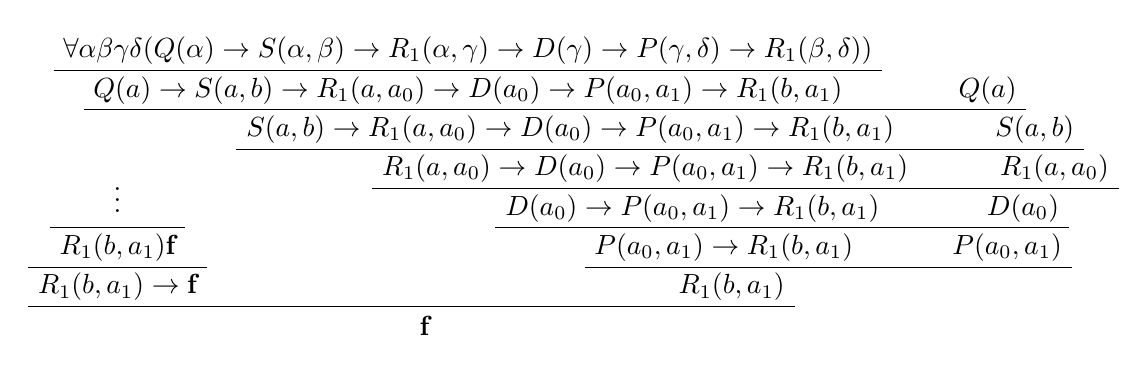
\begin{tikzpicture}[grow=up,level distance=0.5cm,
execute at begin node=$, execute at end node=$,
every node/.style={opacity=1},
every child/.style={edge from parent/.style={opacity=0}}]
\def\dist{0.7cm}
\node(e) {\vdashf \falses} [sibling distance=2*\dist+6.4cm] 
	child {node(1) {\vdashf R_1(b,a_1)} [sibling distance=\dist+2.9cm]
		child[xshift=1.7cm] {node(11) {\vdashf P(a_0,a_1)}}
		child[xshift=1.7cm] {node(12) {\vdashf P(a_0,a_1)\to R_1(b,a_1)} [sibling distance=\dist+3.5cm]
			child[xshift=1.7cm] {node(121) {\vdashf D(a_0)}}
			child[xshift=1.7cm] {node(122) {\vdashf D(a_0)\to P(a_0,a_1)\to R_1(b,a_1)} [sibling distance=\dist+4.5cm]
				child[xshift=2cm] {node(1221) {\vdashf R_1(a,a_0)}}
				child[xshift=2cm] {node(1222) {\vdashf R_1(a,a_0)\to D(a_0)\to P(a_0,a_1)\to R_1(b,a_1)} [sibling distance=\dist+5.2cm]
					child[xshift=2cm] {node(12221) {\vdashf S(a,b)}}
					child[xshift=2cm] {node(12222) {\vdashf S(a,b)\to R_1(a,a_0)\to D(a_0)\to P(a_0,a_1)\to R_1(b,a_1)} [sibling distance=\dist+5.9cm]
						child[xshift=2cm] {node(122221) {\vdashf Q(a)}}
						child[xshift=2cm] {node(122222) {\vdashf Q(a)\to S(a,b)\to R_1(a,a_0)\to D(a_0)\to P(a_0,a_1)\to R_1(b,a_1)}
							child {node(1222221) {\vdashf\forall\alpha\beta\gamma\delta(Q(\alpha)\to S(\alpha,\beta)\to R_1(\alpha,\gamma)\to D(\gamma) \to P(\gamma,\delta)\to R_1(\beta,\delta))}}}}}}}}
	child {node(2) {\vdashf R_1(b,a_1)\to\falses}
		child {node(21) {R_1(b,a_1)\vdashf\falses}
			child {node[label={[yshift=-0.3cm]above:\vdots}](211) {}}}};


%tikz did not want to do this in the loop no idea why
%\coordinate(c1222) at (1222);
%\getwidthofnode{\sright}{12221}
%\draw (c1222)+(-\sright/2,+0.25) -- +(\sright/2,+0.25);

%set of all positions in the tree
\def\nodes{,1,2,11,12,21,121,122,1221,1222,12222,12221,122222,122221,122222,1222221,211}
%the yshift does not work on nodes so we create a coordinate for every node
\foreach \x in \nodes{
\ifnodedefined{\x}{
	\coordinate(c\x) at (\x);
	\coordinate(10.\x) at (0,0);
}{}
}

%draw lines for each node with 2 children (add parents with 2 children)
\foreach \x in \nodes{
\ifnodedefined{10.\x1}{
	%calculate with of line
	\getwidthofnode{\sright}{\x1}
	%if there is a right child draw wide line
	\ifnodedefined{10.\x2}{
		\getwidthofnode{\sleft}{\x2}
		%draw line
		\draw[shorten <=-\sright/2, shorten >=-\sleft/2] ([yshift=-0.25cm]c\x1) -- ([yshift=-0.25cm]c\x2);
	} %else only one child
	{
		\getwidthofnode{\sleft}{\x}
		%get widht corresponding to the widht of the bigger node
		\pgfmathsetlength{\sright}{max(\sright,\sleft)}
		%draw line
		\draw (c\x)+(-\sright/2,+0.25) -- +(\sright/2,+0.25);
	}
}{}
}
\end{tikzpicture}
	\end{figure}
	
	Again it is obvious that we have deduced $\Gamma_D$ ($\widehat{a}:=b$, $\widehat{b}_i:=b_i$ for $i\in\{0,\dots,n\}$, and $\widehat{a}_{i-1}:=a_i$ for $i\in\{1,\dots,m\}$). Hence, by induction hypothesis, we can deduce \false{}.
\end{proof}

\begin{lemma}\label{lem.19}
	\begin{align*} %TODO for any M one can effectively construct? or is M the M from the construction
		  & \text{$M$ terminates on input $(0,0)$} &   & \text{iff} & \text{$\Gamma_M\PModels\false$ holds in system P.} 
	\end{align*}
\end{lemma}
\begin{proof}
	The $\Leftarrow$ directions is proven in Claim \ref{cla.17}. And the $\Rightarrow$ direction is a direct consequence of Claim \ref{cla.18} with $C=\langle Q_0,0,0\rangle$.
\end{proof}

\begin{theorem}
	\PCons{} is undecidable.
\end{theorem}
\begin{proof}
	Since by Lemma \ref{lem.19} for a given two-counter automaton $M$ we can effectively construct a set of \SysP-formulas $\Gamma_M$ such that $M$ terminates on input $(0,0)$ iff $\Gamma_M$ is not consistent. It follows that $\autHalt\leq\PCons$. Since \autHalt{} is undecidable we have shown that \PCons{} is undecidable too.
\end{proof}

	\end{sloppypar}
\end{document}
